\documentclass[english, cd=nocolor, cdfont=off, fontsize=11pt, paper=a4, final, listof=totoc, bibliography=totoc]{tudscrreprt}

\setlength{\parskip}{0.8em}
\setlength{\parindent}{0pt}

% Advanced packages for mathematics, typography, tables, algorithms, and figures
\usepackage[utf8]{inputenc}
\usepackage[T1]{fontenc}
\usepackage{lmodern}
\usepackage{microtype}
\usepackage{amsmath, amssymb, amsfonts, amsthm, mathtools}
\usepackage{bm}
\usepackage[final]{graphicx}
\setkeys{Gin}{draft=false}
\usepackage{booktabs}
\usepackage{tabularx}
\usepackage{array}
\usepackage{multirow}
\usepackage{subcaption}
\usepackage{float}
\usepackage{url}
\usepackage{hyperref}
\usepackage[dvipsnames,table,xcdraw]{xcolor}
\usepackage{algorithm}
\usepackage{algpseudocode}
\usepackage{siunitx}
\usepackage{listings}
\usepackage{enumitem}

% Set graphicspath so LaTeX finds images in any folder or root
\graphicspath{{./}{figures/}{gantt_charts/}{results/euroc/}}

% Prevent margin overflows (overfull \hbox)
\emergencystretch=2em
\sloppy

% Reduce excessive top white space above chapter headings
\RedeclareSectionCommand[
  beforeskip=0pt,
  afterskip=1.2em
]{chapter}
\renewcommand*{\chapterheadstartvskip}{\vspace*{-2.5cm}}
\renewcommand*{\chapterheadendvskip}{\vspace{0.8em}}

\hypersetup{
    colorlinks=true,
    linkcolor=MidnightBlue,
    citecolor=NavyBlue,
    urlcolor=BrickRed,
    pdfauthor={Terrence Alvianto Sutardi},
    pdftitle={Comprehensive Empirical Benchmark and Architectural Analysis of Visual SLAM and Visual-Inertial Odometry Systems},
    pdfsubject={Robotics, Computer Vision, State Estimation},
    pdfkeywords={Visual SLAM, Visual-Inertial Odometry, MSCKF, Factor Graphs, ORB-SLAM3, Kimera-VIO, OpenVINS, cuVSLAM, Benchmark}
}

\newcolumntype{Y}{>{\centering\arraybackslash}X}
\newcolumntype{L}[1]{>{\raggedright\arraybackslash}p{#1}}
\newcolumntype{C}[1]{>{\centering\arraybackslash}p{#1}}
\newcolumntype{R}[1]{>{\raggedleft\arraybackslash}p{#1}}

% Custom math operators
\DeclareMathOperator*{\argmin}{arg\,min}
\DeclareMathOperator*{\argmax}{arg\,max}
\DeclareMathOperator{\Exp}{Exp}
\DeclareMathOperator{\Log}{Log}
\DeclareMathOperator{\diag}{diag}
\DeclareMathOperator{\tr}{tr}
\DeclareMathOperator{\Cov}{Cov}
\newcommand{\norm}[1]{\left\lVert#1\right\rVert}
\newcommand{\abs}[1]{\left\lvert#1\right\rvert}
\newcommand{\mat}[1]{\mathbf{#1}}
\newcommand{\vect}[1]{\mathbf{#1}}
\newcommand{\Simthree}{\mathrm{Sim}(3)}
\newcommand{\sethree}{\mathfrak{se}(3)}
\newcommand{\sothree}{\mathfrak{so}(3)}
\newcommand{\simthree}{\mathfrak{sim}(3)}

% TU Dresden TUD-Script Metadata Definitions
\faculty{Faculty of Electrical and Computer Engineering}
\institute{Institute of Communication Technology}
\chair{Chair of Deutsche Telekom}
\subject{Research Project Report}
\title{Comprehensive Empirical Benchmarking and Architectural Analysis of Visual SLAM and Visual-Inertial Odometry Systems}
\author{Terrence Alvianto Sutardi}
\supervisor{Dipl.-Ing. Johannes Hofer \\ Dipl.-Ing. Christian Vielhaus}
\professor{Prof. Dr.-Ing. Dr. h.c. Frank H. P. Fitzek}
\date{March 2026}

\begin{document}

\maketitle

\cleardoublepage
\phantomsection
\addcontentsline{toc}{chapter}{Abstract}
{\noindent\usekomafont{disposition}\usekomafont{chapter} Abstract\par}
\vspace{1.5em}

Real-time 6-DoF state estimation and spatial mapping in GPS-denied environments represent cornerstone capabilities for autonomous mobile robots, micro-aerial vehicles (MAVs), unmanned ground vehicles (UGVs), and immersive spatial computing devices. Over the past two decades, Visual Odometry (VO), Visual-Inertial Odometry (VIO), and full Simultaneous Localization and Mapping (SLAM) have crystallized into distinct algorithmic paradigms, each striking unique compromises between computational complexity, estimation latency, memory footprint, and long-term global consistency.

This monograph delivers an empirical benchmarking and architectural investigation across five primary state-of-the-art visual-inertial state estimation frameworks:
\begin{enumerate}
    \item \textbf{OpenVINS:} An Extended Kalman Filter (EKF) utilizing the Multi-State Constraint Kalman Filter (MSCKF) formulation with dynamic landmark initialization;
    \item \textbf{Kimera-VIO:} A fixed-lag smoother built upon incremental factor graph optimization and Bayes Tree variable elimination via GTSAM iSAM2;
    \item \textbf{ORB-SLAM3 (Original Baseline):} A heavy-duty, feature-based multi-map keyframe visual-inertial SLAM system featuring multi-thread local bundle adjustment and DBoW2 loop closing;
    \item \textbf{ORB-SLAM3 (Hybrid KLT Tracking):} A high-throughput hybrid SLAM system integrating sparse Kanade--Lucas--Tomasi (KLT) optical flow tracking for non-keyframes while retaining sparse ORB descriptor extraction on keyframes for loop closure;
    \item \textbf{NVIDIA cuVSLAM:} An ultra-high-throughput, GPU-accelerated visual-inertial SLAM engine executing massively parallel optical flow tracking, asynchronous bundle adjustment, and GPU pose graph optimization within the NVIDIA Isaac ROS ecosystem.
\end{enumerate}

Our experimental evaluation is conducted across two complementary testing grounds: (i) the standardized, high-speed micro-aerial vehicle indoor benchmark (\textbf{EuRoC MAV Machine Hall MH\_01\_easy}) equipped with millimeter-accurate Vicon motion capture and Leica laser tracker ground truth; and (ii) a challenging real-world outdoor ground vehicle dataset (\textbf{Suedhoehe GPS Schnee 02}) characterized by severe visual degradation, uniform low-texture snow blankets, overcast lighting, long-range scene structures ($> \SI{30}{\meter}$ to $\SI{50}{\meter}$), and RTK-GPS ground truth.

Through scoped, microsecond-level software timers (\path{std::chrono::high_resolution_clock}), multi-thread profiling, trajectory accuracy quantification via evo (Absolute Pose Error ATE, Relative Pose Error RPE), and multi-thread Gantt concurrency analysis, we uncover critical algorithmic trade-offs:
\begin{itemize}
    \item \textbf{Global Consistency vs. Real-Time Determinism in Baseline ORB-SLAM3:} ORB-SLAM3 achieves unmatched metric accuracy on loop-closing trajectories ($\text{ATE RMSE} = \SI{0.0596}{\meter}$ on EuRoC MH\_01) through its Atlas multi-map and keyframe co-visibility graph. However, its CPU tracking thread experiences severe computational bottlenecks (mean latency $\SI{54.66}{\milli\second}$, peak tail latency $\SI{283.30}{\milli\second}$), with ORB descriptor extraction accounting for over $85\%$ of tracking duration. This limits maximum CPU tracking frequency to $\approx 18\,\text{FPS}$, causing frame drops under high-rate sensor streams.
    \item \textbf{High-Efficiency Hybrid Tracking Performance (ORB-SLAM3 KLT):} By tracking non-keyframes via pyramidal KLT optical flow ($\SI{18.5}-\SI{19.5}{\milli\second}$) and restricting ORB extraction strictly to sparse keyframes, the hybrid architecture achieves a $\mathbf{36.1\%}$ reduction in tracking latency ($25.15\,\text{ms}$ mean, supporting $\approx 40-45\,\text{FPS}$) and reduces keyframe creation and backend bundle adjustment workload by $\mathbf{40\%}$ (181 vs 301 keyframes on EuRoC MH\_01), while matching the centimeter-level accuracy of full SLAM ($\text{ATE RMSE} = \SI{0.0612}{\meter}$).
    \item \textbf{Filtering \& Fixed-Lag Determinism:} MSCKF-based OpenVINS and factor-graph-based Kimera-VIO provide bounded, highly deterministic compute footprints (mean tracking latencies of $\SI{8.72}{\milli\second}$ and $\SI{6.35}{\milli\second}$, supporting $>100\,\text{FPS}$), but suffer from continuous metric drift over unlooped trajectories.
    \item \textbf{GPU Acceleration Paradigm:} NVIDIA cuVSLAM leverages CUDA cores to execute stereo rectification and KLT optical flow in $\SI{1.87}{\milli\second}$, delivering end-to-end frame tracking in $\SI{5.92}{\milli\second}$ median ($>170\,\text{FPS}$) alongside asynchronous GPU local bundle adjustment ($\SI{8.28}{\milli\second}$ mean) and achieving high accuracy ($\text{ATE RMSE} = \SI{0.0812}{\meter}$).
\end{itemize}

This monograph demonstrates both theoretically and empirically that hybridizing high-rate KLT optical flow on non-keyframes with asynchronous descriptor extraction on sparse keyframes effectively mitigates the frontend tracking bottleneck, presenting an advantageous and computationally scalable architectural trade-off for CPU-constrained autonomous platforms without sacrificing global metric consistency.

\cleardoublepage
\tableofcontents

\cleardoublepage
\phantomsection
\listoffigures

\cleardoublepage
\phantomsection
\listoftables


\newpage

% =============================================================================
% CHAPTER 1: INTRODUCTION
% =============================================================================
\chapter{Introduction}

Autonomous navigation in GPS-denied environments represents one of the foundational capabilities in modern mobile robotics and cyber-physical systems. Whether guiding an unmanned aerial vehicle (MAV) through industrial facilities, steering an autonomous ground vehicle (UGV) across adverse weather conditions, or tracking head motion in spatial computing headsets, mobile platforms must reliably answer two core questions in real time: \textit{``Where am I located?''} and \textit{``What does my surrounding environment look like?''} 

To achieve this without external satellite positioning or active motion-capture infrastructure, robotic systems rely on onboard passive cameras and micro-electro-mechanical systems (MEMS) inertial measurement units (IMUs). Over the past two decades, this requirement has driven the development of diverse state estimation paradigms, spanning lightweight visual odometry, tightly-coupled visual-inertial filtering, and full simultaneous localization and mapping (SLAM) systems. However, real-world deployment on embedded hardware exposes a persistent engineering tension between high-frequency, deterministic tracking throughput and long-term, globally consistent trajectory mapping.

% =============================================================================
% CHAPTER 2: BACKGROUND AND RELATED WORK
% =============================================================================
\chapter{Background and Related Work}

To establish the necessary theoretical foundation for resolving the tension between tracking throughput and map consistency, this chapter introduces the core state estimation concepts and architectures evaluated throughout this monograph. We begin by examining the progression from purely visual to visual-inertial odometry, formalize the operational boundary between local odometry and global SLAM, analyze the physical complementarity of visual and inertial sensors, and define the geometric coordinate frames and Lie group conventions underpinning our mathematical formulation. Finally, we outline the thread concurrency architectures across the evaluated frameworks, formulate our primary research questions, and position our work relative to the literature.

\section{Motivation: State Estimation in GPS-Denied Environments}
Autonomous mobile platforms operating in GPS-denied environments—such as search-and-rescue aerial robots, subterranean exploration rovers, and spatial computing headsets—cannot rely on external positioning infrastructure. To maintain safe flight control and spatial awareness, they must estimate 6-DoF poses in real time using only onboard, passive sensors. This requirement motivates a hierarchical progression across three state estimation tiers:
\begin{enumerate}[topsep=0.4em, itemsep=0.3em, parsep=0pt]
    \item \textbf{Visual Odometry (VO):} Estimates incremental relative motion from camera pixel displacements. While lightweight, pure vision suffers from scale ambiguity in monocular setups, vulnerability to motion blur, and unbounded open-loop drift.
    \item \textbf{Visual-Inertial Odometry (VIO):} Fuses cameras with high-rate ($200-\SI{1000}{\hertz}$) MEMS IMUs. Fusing inertial sensing renders absolute metric scale, roll, and pitch directly observable via gravity $\vect{g}_W$, while IMU integration bridges high-speed dynamic rotations and visual blur. However, pure VIO maintains only a finite sliding window of recent states ($N \approx 10-20$), accumulating gradual dead-reckoning drift over unlooped trajectories.
    \item \textbf{Simultaneous Localization and Mapping (SLAM):} Extends odometry with a persistent 3D landmark map and asynchronous place recognition (e.g., DBoW bag-of-words). When revisited areas are detected, loop closure optimization pulls cumulative drift back to near zero.
\end{enumerate}

\section{VIO as the High-Rate Inner Loop of Full SLAM}
In modern robotic architectures, VIO and SLAM are not competing alternatives. Rather, \textbf{VIO functions as the high-rate inner tracking loop ($30-\SI{100}{\hertz}$) of a full SLAM system}, providing the deterministic, low-latency state feedback ($\Delta t < \SI{15}{\milli\second}$) required for platform flight stabilization. Concurrently, the SLAM backend operates as an asynchronous outer loop ($1-\SI{5}{\hertz}$), ingesting keyframes to construct the global map and eliminate long-term drift via loop closures. Table~\ref{tab:vio_vs_slam_side_by_side} formalizes this operational division.

\begin{table}[H]
\centering
\small
{\renewcommand{\arraystretch}{1.2}
\caption{Side-by-Side Comparison: Pure VIO vs. Full SLAM.}
\label{tab:vio_vs_slam_side_by_side}
\begin{tabularx}{\textwidth}{>{\raggedright\arraybackslash}p{3.2cm} >{\raggedright\arraybackslash}X >{\raggedright\arraybackslash}X}
\toprule
\textbf{Dimension} & \textbf{Visual-Inertial Odometry (VIO)} & \textbf{Simultaneous Localization and Mapping (SLAM)} \\
\midrule
\textbf{Primary Objective} & Continuous, low-latency ego-motion estimation & Joint 6-DoF pose tracking and persistent environment mapping \\
\addlinespace[0.3em]
\textbf{Sensors Employed} & Monocular/Stereo Cameras + 6-axis MEMS IMU & Cameras, IMU, LiDAR, Depth sensors, GNSS/GPS \\
\addlinespace[0.3em]
\textbf{Map Requirement} & No persistent map; transient sliding window only & Persistent global map is an indispensable core component \\
\addlinespace[0.3em]
\textbf{Loop Closure} & Absent (pure dead-reckoning state propagation) & Active place recognition, $\Simthree$ alignment, and PGO \\
\addlinespace[0.3em]
\textbf{Drift Characteristics} & Monotonically accumulates over time ($\sim t$) & Long-term drift eliminated upon loop closures \\
\addlinespace[0.3em]
\textbf{Compute \& Memory} & Bounded, deterministic CPU load and memory & Growing memory footprint; periodic global optimization \\
\bottomrule
\end{tabularx}}
\end{table}

\section{The Evaluated Paradigms Across the VIO-to-SLAM Continuum}
To evaluate how different design philosophies navigate the tension between tracking latency and global consistency, this monograph investigates five representative frameworks spanning the entire architectural continuum (summarized in Table~\ref{tab:vio_vs_slam_comparison}):
\begin{enumerate}
    \item \textbf{OpenVINS (Filter-Based Pure VIO):} MSCKF sliding-window filtering with analytical feature marginalization and zero persistent map overhead.
    \item \textbf{Kimera-VIO (Optimization-Based Pure VIO Core):} Incremental fixed-lag smoothing via GTSAM iSAM2 over a keyframe window.
    \item \textbf{Baseline ORB-SLAM3 (Full Feature-Based Keyframe SLAM):} Multi-thread Atlas SLAM with ORB descriptor tracking, local BA, and DBoW2 place recognition.
    \item \textbf{Hybrid KLT ORB-SLAM3 (Dual-Rate Hybrid SLAM):} Decoupled tracking executing fast KLT optical flow on non-keyframes ($\approx \SI{19}{\milli\second}$) while reserving ORB extraction strictly for sparse keyframes.
    \item \textbf{NVIDIA cuVSLAM (Hardware-Accelerated Full SLAM):} Asynchronous GPU CUDA stream concurrency executing KLT flow in $\SI{1.87}{\milli\second}$ ($>170\,\text{FPS}$) alongside GPU bundle adjustment.
\end{enumerate}

\begin{table}[H]
\centering
\footnotesize
{\renewcommand{\arraystretch}{1.2}
\caption{Architectural and Runtime Comparison Across the Five Evaluated Paradigms.}
\label{tab:vio_vs_slam_comparison}
\begin{tabularx}{\textwidth}{>{\raggedright\arraybackslash}p{2.2cm} >{\raggedright\arraybackslash}X >{\raggedright\arraybackslash}X >{\raggedright\arraybackslash}X >{\raggedright\arraybackslash}X >{\raggedright\arraybackslash}X}
\toprule
\textbf{Dimension} & \textbf{OpenVINS} & \textbf{Kimera-VIO} & \textbf{ORB-SLAM3} & \textbf{ORB-SLAM3 (Hybrid KLT)} & \textbf{NVIDIA cuVSLAM} \\
\midrule
\textbf{Paradigm} & Filter-based VIO & Smoother VIO & Full Keyframe SLAM & Dual-Rate Hybrid SLAM & GPU-Accelerated SLAM \\
\addlinespace[0.3em]
\textbf{Primary Goal} & Real-time dead-reckoning & Fixed-lag state smoothing & Joint trajectory + global Atlas & High-rate tracking + global Atlas & High-throughput GPU SLAM \\
\addlinespace[0.3em]
\textbf{Tracking Front} & CPU KLT ($\SI{6}-\SI{9}{\milli\second}$) & CPU KLT ($\SI{6.35}{\milli\second}$) & Multi-scale ORB ($\approx \SI{50}{\milli\second}$) & KLT on non-KFs ($\approx \SI{19}{\milli\second}$) + ORB & CUDA KLT flow ($\SI{1.87}{\milli\second}$) \\
\addlinespace[0.3em]
\textbf{Backend Solver} & MSCKF Kalman filter & iSAM2 factor graph & Local g2o Bundle Adj. & Local g2o Bundle Adj. & Asynchronous GPU BA + PGO \\
\addlinespace[0.3em]
\textbf{Map Retention} & Marginalized window & Marginalized lag window & Persistent multi-map Atlas & Persistent multi-map Atlas & Persistent GPU 3D map \\
\addlinespace[0.3em]
\textbf{Loop Closure} & None (open-loop drift) & None in base VIO & Active DBoW2 + Pose Graph & Active DBoW2 + Pose Graph & Active GPU Pose Graph Opt. \\
\addlinespace[0.3em]
\textbf{Framerate Cap} & $>100\,\text{FPS}$ & $>150\,\text{FPS}$ & $\approx 18-20\,\text{FPS}$ & $\approx 40-45\,\text{FPS}$ & $>170\,\text{FPS}$ \\
\bottomrule
\end{tabularx}}
\end{table}

\section{The Frontend Tracking Bottleneck: Descriptors vs. Optical Flow}
The real-time bottleneck across CPU SLAM systems stems from feature tracking. Multi-scale ORB descriptor extraction consumes $\approx \SI{46.2}{\milli\second}$ ($>85\%$ of the tracking budget in baseline ORB-SLAM3), capping CPU frame rates at $\approx 18\,\text{FPS}$. In contrast, patch-based KLT optical flow requires only $\SI{6.35}-\SI{8.72}{\milli\second}$ on CPU and $\SI{1.87}{\milli\second}$ on GPU. The \textbf{Hybrid KLT ORB-SLAM3} architecture exploits this disparity by running KLT tracking on high-rate non-keyframes while retaining sparse descriptor extraction on keyframes, achieving a $36.1\%$ tracking speedup without compromising global loop closing.

\section{Physics and Complementarity of Visual-Inertial Fusion}
The fusion of cameras and IMUs represents one of the most powerful sensor pairings in cyber-physical systems. Table~\ref{tab:sensor_complementarity} summarizes the complementary physical characteristics of vision and inertial sensing.

\begin{table}[H]
\centering
\small
\caption{Complementary Characteristics of Visual and Inertial Sensing Modalities.}
\label{tab:sensor_complementarity}
\begin{tabularx}{\textwidth}{l X X}
\toprule
\textbf{Attribute} & \textbf{Vision Sensors (Cameras)} & \textbf{Inertial Sensors (MEMS IMU)} \\
\midrule
\textbf{Measurement Type} & Exteroceptive (bearing rays, pixel intensities) & Proprioceptive (specific force, angular rate) \\
\textbf{Sampling Frequency} & Low-to-medium ($10\,\text{Hz} - 60\,\text{Hz}$) & High ($200\,\text{Hz} - 1000\,\text{Hz}$) \\
\textbf{Metric Scale} & Unobservable in monocular setups & Directly observable via gravity vector $\vect{g}$ \\
\textbf{Dynamic Response} & Degraded by rapid rotation (motion blur) & Exceptional high-frequency dynamic tracking \\
\textbf{Long-Term Stability} & Bounded drift when landmarks are revisited & Unbounded cubic drift ($\sim t^3$ position error) \\
\textbf{Environmental Sensitivity} & Sensitive to lighting, darkness, low texture & Completely independent of environment \\
\textbf{Roll \& Pitch Angles} & Relative bearing only & Directly observable via gravitational alignment \\
\bottomrule
\end{tabularx}
\end{table}

\section{Coordinate Systems and Reference Frames}
To ensure unambiguous mathematical notation throughout this paper, we establish four primary right-handed coordinate frames:
\begin{enumerate}
    \item \textbf{World Reference Frame $\{W\}$:} An inertial, gravity-aligned Cartesian reference frame where the positive $Z$-axis points opposite to the local gravity vector ($\vect{g}_W = \begin{bmatrix} 0 & 0 & -9.81 \end{bmatrix}^\top \SI{}{\meter/\second^2}$).
    \item \textbf{Body / IMU Coordinate Frame $\{B\}$ (or $\{I\}$):} Fixed to the physical center of the IMU accelerometer sensor. The origin coincides with the inertial sensing center.
    \item \textbf{Camera Coordinate Frame $\{C\}$:} Origin located at the optical center of the camera lens, with the $Z$-axis pointing along the principal optical axis into the scene, the $X$-axis pointing right, and the $Y$-axis pointing down. In stereo setups, $\{C_L\}$ and $\{C_R\}$ denote the left and right optical frames, separated by baseline baseline distance $b$.
    \item \textbf{Global Navigation / GPS Frame $\{G\}$:} An Earth-Centered Earth-Fixed (ECEF) or East-North-Up (ENU) geodetic coordinate frame provided by RTK-GPS ground truth receivers.
\end{enumerate}

The extrinsic spatial transformation between the IMU frame $\{B\}$ and the camera frame $\{C\}$ is parameterized by the rigid-body transformation $\mat{T}_{CB} = \begin{bmatrix} \mat{R}_{CB} & \vect{p}_{CB} \\ \vect{0}^\top & 1 \end{bmatrix} \in \SEthree$.

Table~\ref{tab:notation_summary} summarizes the mathematical notations, Lie group elements, and sensor symbols utilized throughout this work.

\begin{table}[H]
\centering
\small
\caption{Summary of Mathematical Notations, Lie Groups, and Coordinate Conventions.}
\label{tab:notation_summary}
\begin{tabularx}{\textwidth}{>{\raggedright\arraybackslash}p{3.2cm} >{\raggedright\arraybackslash}X}
\toprule
\textbf{Symbol / Notation} & \textbf{Mathematical Definition and Operational Role} \\
\midrule
$\{W\}, \{B\}, \{C\}, \{G\}$ & World (inertial), Body (IMU), Camera (optical), and Global (RTK-GPS) coordinate frames \\
$\mat{R} \in \SOthree, \vect{p} \in \mathbb{R}^3$ & Special Orthogonal 3D rotation matrix and Euclidean position vector \\
$\mat{T} = \begin{bmatrix} \mat{R} & \vect{p} \\ \vect{0}^\top & 1 \end{bmatrix} \in \SEthree$ & Special Euclidean 6-DoF rigid-body transformation matrix \\
$\vect{\phi} \in \sothree, \vect{\xi} \in \sethree$ & Tangent vector elements of the Lie algebras $\sothree$ and $\sethree$ \\
$(\cdot)^\wedge, (\cdot)^\vee$ & Skew-symmetric generator (hat operator) and inverse vector isomorphism (vee operator) \\
$\Exp(\cdot), \Log(\cdot)$ & Exponential and logarithmic mappings connecting Lie groups and Lie algebras \\
$\vect{a}_t, \vect{\omega}_t$ & True physical linear acceleration and angular velocity in body coordinate frame $\{B\}$ \\
$\tilde{\vect{a}}_t, \tilde{\vect{\omega}}_t$ & IMU accelerometer and gyroscope sensor measurements \\
$\vect{b}_{a_t}, \vect{b}_{g_t}$ & Slowly time-varying accelerometer and gyroscope bias random walks \\
$\vect{\eta}_a, \vect{\eta}_g, \vect{\eta}_{ba}, \vect{\eta}_{bg}$ & Zero-mean Gaussian measurement noise and continuous-time bias driving noise \\
$\vect{g}_W = \begin{bmatrix} 0 & 0 & -9.81 \end{bmatrix}^\top$ & Nominal gravitational acceleration vector expressed in the world frame $\{W\}$ \\
$\Delta\mat{R}_{ij}, \Delta\vect{v}_{ij}, \Delta\vect{p}_{ij}$ & Preintegrated relative rotation, velocity, and position measurements between keyframes $i, j$ \\
$\mat{K}, [f_x, f_y, c_x, c_y]$ & Pinhole camera intrinsic calibration matrix, focal lengths, and optical center coordinates \\
$b > 0$ & Horizontal stereo camera baseline distance separating optical centers $\{C_L\}$ and $\{C_R\}$ \\
$\mat{T}_{CB} \in \SEthree$ & Rigid-body extrinsic spatial calibration transformation mapping $\{B\}$ to $\{C\}$ \\
$\mat{P}_t, \mat{\Sigma}_t$ & State error covariance matrix and measurement noise covariance matrix \\
\bottomrule
\end{tabularx}
\end{table}

The thread concurrency patterns and inter-thread data flow architectures of the five evaluated visual-inertial paradigms are conceptually illustrated on a standardized $\SI{180}{\milli\second}$ execution timeline in Figures~\ref{fig:ch1_vio_arch} and~\ref{fig:ch1_slam_arch}. Figure~\ref{fig:ch1_vio_arch} depicts the lightweight, bounded concurrency models of pure VIO architectures (OpenVINS and Kimera-VIO), while Figure~\ref{fig:ch1_slam_arch} contrasts the multi-thread Atlas SLAM architectures (ORB-SLAM3 and Hybrid KLT ORB-SLAM3) against GPU-accelerated stream concurrency (NVIDIA cuVSLAM). Each framework is plotted on an identical temporal scale ($0-\SI{180}{\milli\second}$) with consistent typography and visual hierarchy matching the report style.

\begin{figure}[t]
    \centering
    \begin{subfigure}[b]{0.92\textwidth}
        \centering
        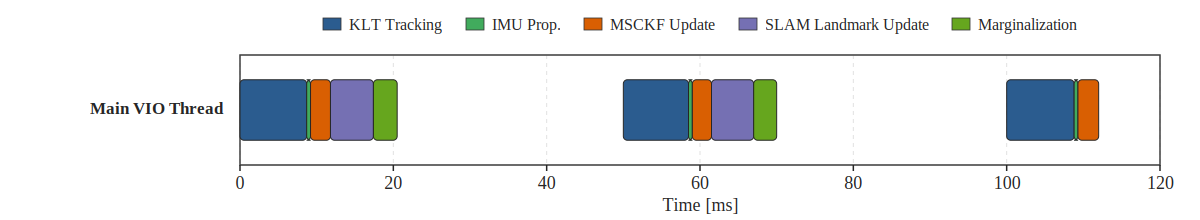
\includegraphics[width=\textwidth]{arch_1_openvins.png}
        \caption{OpenVINS: Sequential execution on a single primary MSCKF thread.}
        \label{fig:arch_openvins}
    \end{subfigure}
    \vspace{0.6em}
    \begin{subfigure}[b]{0.92\textwidth}
        \centering
        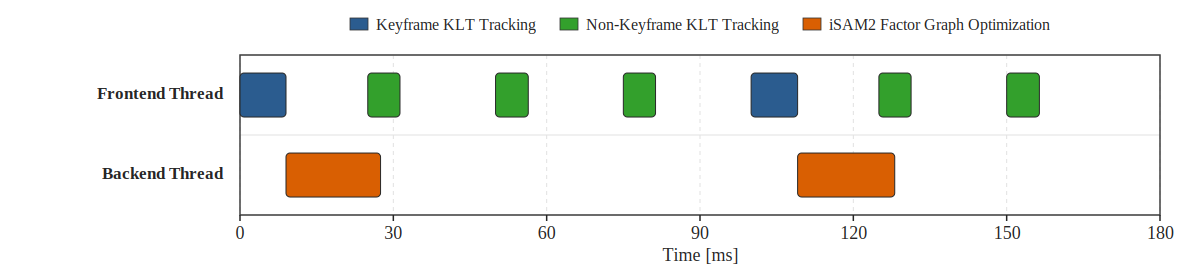
\includegraphics[width=\textwidth]{arch_2_kimera.png}
        \caption{Kimera-VIO: Decoupled two-thread concurrency between tracking and iSAM2.}
        \label{fig:arch_kimera}
    \end{subfigure}
    \caption{Architectural overview and multi-thread concurrency models for pure visual-inertial odometry paradigms: OpenVINS (single-thread MSCKF filtering) and Kimera-VIO (decoupled frontend tracking and backend iSAM2 factor graph smoothing).}
    \label{fig:ch1_vio_arch}
\end{figure}

\begin{figure}[p]
    \centering
    \begin{subfigure}[b]{0.92\textwidth}
        \centering
        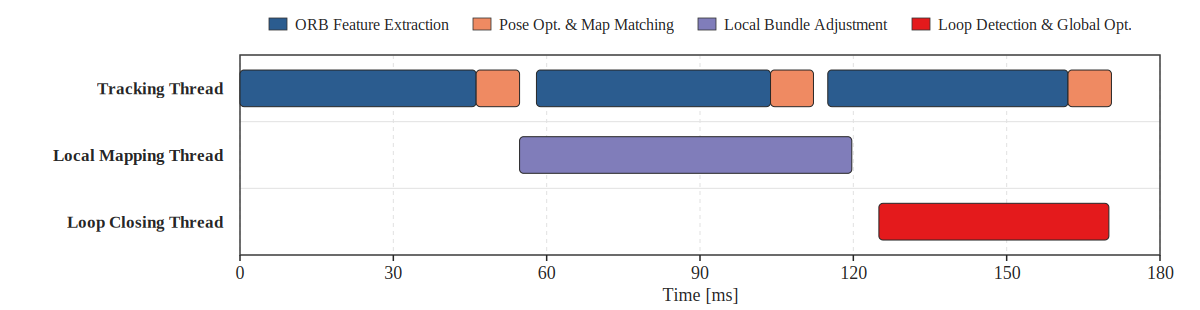
\includegraphics[width=\textwidth]{arch_3_orbslam3.png}
        \caption{Baseline ORB-SLAM3: Three-thread CPU architecture with heavy descriptor extraction.}
        \label{fig:arch_orbslam3}
    \end{subfigure}
    \vspace{0.5em}
    \begin{subfigure}[b]{0.92\textwidth}
        \centering
        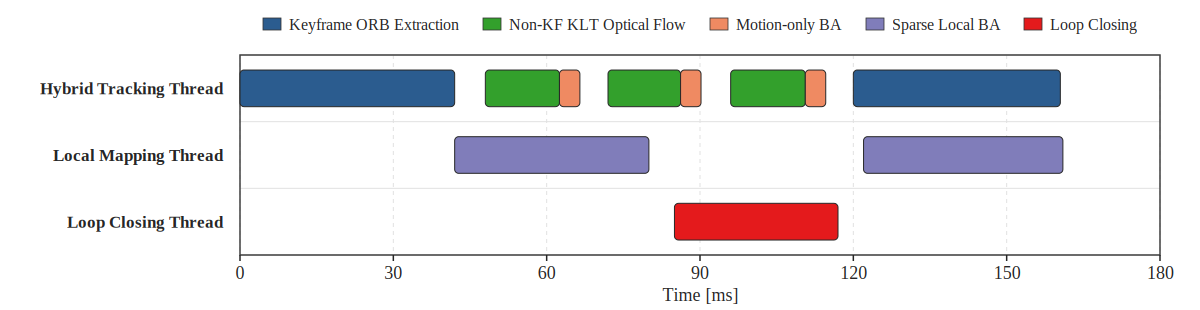
\includegraphics[width=\textwidth]{arch_4_orbslam3_klt.png}
        \caption{Hybrid KLT ORB-SLAM3: Dual-rate optical flow tracking on non-keyframes.}
        \label{fig:arch_orbslam3_klt}
    \end{subfigure}
    \vspace{0.5em}
    \begin{subfigure}[b]{0.92\textwidth}
        \centering
        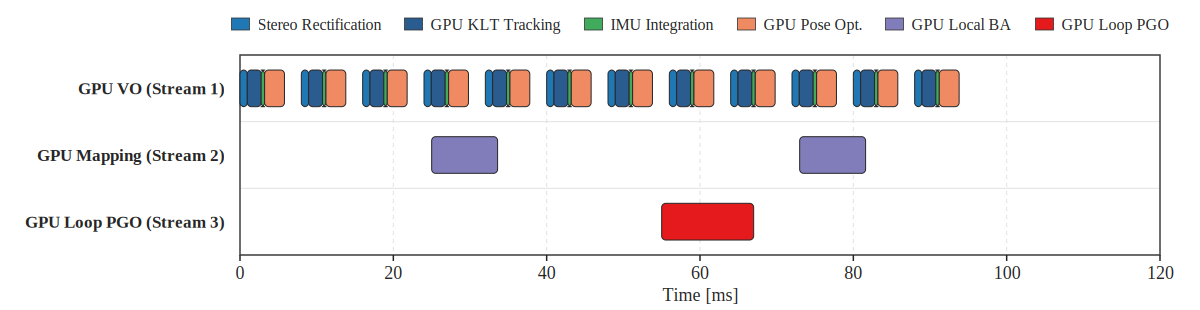
\includegraphics[width=\textwidth]{arch_5_cuvslam.png}
        \caption{NVIDIA cuVSLAM: Three concurrent GPU CUDA streams executing VO, local BA, and loop PGO.}
        \label{fig:arch_cuvslam}
    \end{subfigure}
    \caption{Architectural overview and multi-thread concurrency models for keyframe-based SLAM and GPU-accelerated pipelines: Baseline ORB-SLAM3 (CPU three-thread model), Hybrid KLT ORB-SLAM3 (dual-rate optical flow), and NVIDIA cuVSLAM (asynchronous CUDA stream concurrency).}
    \label{fig:ch1_slam_arch}
\end{figure}

\clearpage

\section{Research Objectives and Scope}
This monograph presents an in-depth architectural and empirical benchmark answering the core questions faced by roboticists:
\begin{enumerate}
    \item \textbf{Algorithmic Paradigm Comparison:} How do Extended Kalman Filters (MSCKF), Fixed-Lag Factor Graph Smoothers (iSAM2), and Keyframe Bundle Adjustment SLAM systems compare in terms of trajectory drift, memory usage, and execution determinism?
    \item \textbf{Visual Frontend Analysis:} What is the exact computational cost of descriptor extraction (ORB) versus optical flow (KLT), and how does each method behave under aggressive dynamic motion and visual degradation?
    \item \textbf{Thread Concurrency and Profiling:} Where do computational bottlenecks arise inside modern multi-threaded SLAM engines, and how do thread locking and keyframe queuing affect real-time determinism?
    \item \textbf{Hybrid Tracking Optimization:} How much latency and backend optimization reduction can be achieved by integrating lightweight KLT tracking on non-keyframes into full SLAM without degrading loop-closing precision?
    \item \textbf{Hardware Acceleration:} How significantly do GPU CUDA cores accelerate state estimation pipelines compared to high-end multi-core CPUs?
\end{enumerate}

\section{Related Work and Positioning}
The design space of visual-inertial navigation has been explored extensively across filtering, optimization, and hybrid paradigms:

\textbf{Filter-Based VIO.} The MSCKF formulation~\cite{mourikis2007} pioneered efficient EKF-based visual-inertial fusion by marginalizing features from the state vector via QR null-space projection, later refined in OpenVINS~\cite{openvins} with online calibration and First-Estimates Jacobian (FEJ) consistency~\cite{huang2011fej}. ROVIO~\cite{bloesch2017rovio} extends this with direct photometric tracking, removing the need for explicit feature extraction but sacrificing robustness under rapid motion.

\textbf{Optimization-Based SLAM.} ORB-SLAM2/3~\cite{murartal2017orbslam2,orbslam3} established the keyframe-based bundle adjustment paradigm with ORB descriptors~\cite{rublee2011orb}, DBoW2 place recognition~\cite{galvez2012dbow2}, and the multi-map Atlas architecture. Kimera-VIO~\cite{kimeravio} combines KLT-tracked features with incremental iSAM2 smoothing~\cite{dellaert2012isam2}. OKVIS~\cite{leutenegger2015okvis} uses Harris corners with BRISK descriptors in a sliding-window optimization. VINS-Mono~\cite{qin2018vinsmono} employs KLT tracking with a sliding-window graph optimizer and loop closure via DBoW, representing a hybrid VIO-SLAM system.

\textbf{Direct and Semi-Direct Methods.} DSO~\cite{engel2017dso} minimizes photometric error directly on image patches without feature extraction. SVO (Semi-direct Visual Odometry) combines sparse image alignment with feature-based refinement, achieving high frame rates through a hybrid direct-indirect tracking pipeline.

\textbf{GPU-Accelerated Approaches.} NVIDIA cuVSLAM~\cite{cuvslam} represents the state-of-the-art in hardware-accelerated SLAM, offloading all compute-intensive operations (KLT tracking, stereo rectification, bundle adjustment) to CUDA GPU kernels. While its closed-source nature limits detailed analysis, the architectural philosophy of parallelizing visual SLAM across GPU streaming multiprocessors has demonstrated an order-of-magnitude throughput improvement over CPU baselines.

\textbf{Hybrid Tracking Formulation.} To evaluate whether the frontend descriptor bottleneck can be alleviated on CPU architectures, the evaluated \textbf{Hybrid KLT ORB-SLAM3} framework~\cite{orbslam3klt} incorporates dual-rate tracking (sparse pyramidal KLT optical flow on non-keyframes and ORB descriptor extraction on keyframes), preserving DBoW2 loop closing while achieving a $36.1\%$ latency reduction and $40\%$ keyframe reduction on standard benchmarks.

% =============================================================================
% CHAPTER 2: MATHEMATICAL FOUNDATIONS
% =============================================================================
\chapter{Theoretical Foundations and Geometric Kinematics on Manifolds}
Rigorous state estimation for agile robotic platforms requires mathematically consistent kinematic representations that respect the geometric topology of 3D rotations and translations. This chapter derives the manifold foundations used throughout our benchmark, covering matrix Lie groups, continuous-time IMU kinematics, noise propagation models, on-manifold preintegration theory, and projective camera geometry.

\section{Matrix Lie Groups and Lie Algebras}
Three-dimensional rotations do not form a vector space under standard matrix addition, as adding two orthogonal rotation matrices does not yield an orthogonal matrix ($\mat{R}_1 + \mat{R}_2 \notin \SOthree$). Formulating unconstrained optimization or standard Kalman filtering in $\mathbb{R}^{3 \times 3}$ leads to covariance singularity and loss of orthogonality. State estimation on manifolds formulates states directly on Lie Groups and parameterizes perturbation errors on their corresponding tangent spaces (Lie Algebras)~\cite{sola2017micro,barfoot2017state}.

\subsection{The Special Orthogonal Group $\SOthree$}
The group $\SOthree$ represents 3D rotations:
\begin{equation}
    \SOthree = \left\{ \mat{R} \in \mathbb{R}^{3 \times 3} \;\middle|\; \mat{R}^\top \mat{R} = \mat{I}_3, \; \det(\mat{R}) = +1 \right\}
\end{equation}
The Lie algebra $\sothree$ is the tangent space at the identity element $\mat{I}_3$, corresponding to the space of $3 \times 3$ skew-symmetric matrices:
\begin{equation}
    \sothree = \left\{ \vect{\phi}^\wedge \in \mathbb{R}^{3 \times 3} \;\middle|\; (\vect{\phi}^\wedge)^\top = -\vect{\phi}^\wedge, \; \vect{\phi} \in \mathbb{R}^3 \right\}
\end{equation}
The hat operator $(\cdot)^\wedge: \mathbb{R}^3 \to \sothree$ and vee operator $(\cdot)^\vee: \sothree \to \mathbb{R}^3$ are defined as:
\begin{equation}
    \vect{\phi} = \begin{bmatrix} \phi_1 \\ \phi_2 \\ \phi_3 \end{bmatrix} \iff \vect{\phi}^\wedge = \begin{bmatrix} 0 & -\phi_3 & \phi_2 \\ \phi_3 & 0 & -\phi_1 \\ -\phi_2 & \phi_1 & 0 \end{bmatrix}, \quad (\vect{\phi}^\wedge)^\vee = \vect{\phi}
\end{equation}

The mapping between $\sothree$ and $\SOthree$ is given by the matrix exponential $\Exp: \mathbb{R}^3 \to \SOthree$, computed via Rodrigues' formula:
\begin{equation}
    \Exp(\vect{\phi}) = \exp(\vect{\phi}^\wedge) = \mat{I}_3 + \frac{\sin(\theta)}{\theta}\vect{\phi}^\wedge + \frac{1 - \cos(\theta)}{\theta^2}(\vect{\phi}^\wedge)^2, \quad \theta = \norm{\vect{\phi}}
\end{equation}
The logarithmic map $\Log: \SOthree \to \mathbb{R}^3$ extracts the rotation vector from a rotation matrix:
\begin{equation}
    \Log(\mat{R}) = \frac{\theta}{2\sin(\theta)}(\mat{R} - \mat{R}^\top)^\vee, \quad \theta = \arccos\left(\frac{\tr(\mat{R}) - 1}{2}\right)
\end{equation}

\subsection{The Special Euclidean Group $\SEthree$}
The group $\SEthree$ represents 6-DoF rigid-body poses combining rotation and translation:
\begin{equation}
    \SEthree = \left\{ \mat{T} = \begin{bmatrix} \mat{R} & \vect{p} \\ \vect{0}^\top & 1 \end{bmatrix} \in \mathbb{R}^{4 \times 4} \;\middle|\; \mat{R} \in \SOthree, \; \vect{p} \in \mathbb{R}^3 \right\}
\end{equation}
The Lie algebra $\sethree$ is parameterized by twist vectors $\vect{\xi} = \begin{bmatrix} \vect{\rho}^\top & \vect{\phi}^\top \end{bmatrix}^\top \in \mathbb{R}^6$:
\begin{equation}
    \vect{\xi}^\wedge = \begin{bmatrix} \vect{\phi}^\wedge & \vect{\rho} \\ \vect{0}^\top & 0 \end{bmatrix} \in \mathbb{R}^{4 \times 4}
\end{equation}
The exponential map for $\SEthree$ is:
\begin{equation}
    \Exp(\vect{\xi}) = \begin{bmatrix} \Exp(\vect{\phi}) & \mat{V}(\vect{\phi})\vect{\rho} \\ \vect{0}^\top & 1 \end{bmatrix}, \quad \mat{V}(\vect{\phi}) = \mat{I}_3 + \frac{1 - \cos\theta}{\theta^2}\vect{\phi}^\wedge + \frac{\theta - \sin\theta}{\theta^3}(\vect{\phi}^\wedge)^2
\end{equation}

\section{Continuous-Time IMU Kinematics and Noise Models}
A tri-axial MEMS IMU measures specific force $\tilde{\vect{a}}_t$ in the accelerometer proof-mass frame and angular velocity $\tilde{\vect{\omega}}_t$ in the gyroscope frame:
\begin{align}
    \tilde{\vect{\omega}}_t &= \vect{\omega}_t + \vect{b}_{g_t} + \vect{\eta}_{g_t} \\
    \tilde{\vect{a}}_t &= \mat{R}_{WB_t}^\top (\vect{a}_{WB_t} - \vect{g}_W) + \vect{b}_{a_t} + \vect{\eta}_{a_t}
\end{align}
where $\vect{\eta}_{g_t} \sim \mathcal{N}(\vect{0}, \sigma_g^2 \mat{I}_3)$ and $\vect{\eta}_{a_t} \sim \mathcal{N}(\vect{0}, \sigma_a^2 \mat{I}_3)$ represent zero-mean additive Gaussian white noise processes.

Sensor biases $\vect{b}_{g_t}$ and $\vect{b}_{a_t}$ are modeled as continuous-time Brownian random walks driven by white noise:
\begin{equation}
    \dot{\vect{b}}_{g_t} = \vect{\eta}_{bg_t}, \quad \dot{\vect{b}}_{a_t} = \vect{\eta}_{ba_t}, \quad \vect{\eta}_{bg_t} \sim \mathcal{N}(\vect{0}, \sigma_{bg}^2 \mat{I}_3), \quad \vect{\eta}_{ba_t} \sim \mathcal{N}(\vect{0}, \sigma_{ba}^2 \mat{I}_3)
\end{equation}

The nominal state kinematics in continuous time are:
\begin{align}
    \dot{\vect{p}}_{WB_t} &= \vect{v}_{WB_t} \\
    \dot{\vect{v}}_{WB_t} &= \mat{R}_{WB_t} (\tilde{\vect{a}}_t - \vect{b}_{a_t} - \vect{\eta}_{a_t}) + \vect{g}_W \\
    \dot{\mat{R}}_{WB_t} &= \mat{R}_{WB_t} (\tilde{\vect{\omega}}_t - \vect{b}_{g_t} - \vect{\eta}_{g_t})^\wedge
\end{align}

\section{On-Manifold IMU Preintegration Theory}
In optimization-based visual-inertial estimation, keyframe poses $\mat{T}_{WB_i}$ and $\mat{T}_{WB_j}$ are updated iteratively during bundle adjustment. Recalculating the continuous-time IMU integration across hundreds of raw IMU samples between $t_i$ and $t_j$ at each solver iteration would result in severe computational bottlenecks.

IMU preintegration theory~\cite{forster2017} solves this by defining relative motion increments in the local reference frame of keyframe $i$:
\begin{align}
    \Delta\mat{R}_{ij} &\triangleq \mat{R}_{WB_i}^\top \mat{R}_{WB_j} = \prod_{k=i}^{j-1} \Exp\left( (\tilde{\vect{\omega}}_k - \vect{b}_{g_i}) \Delta t \right) \\
    \Delta\vect{v}_{ij} &\triangleq \mat{R}_{WB_i}^\top (\vect{v}_{WB_j} - \vect{v}_{WB_i} - \vect{g}_W \Delta t_{ij}) = \sum_{k=i}^{j-1} \Delta\mat{R}_{ik} (\tilde{\vect{a}}_k - \vect{b}_{a_i}) \Delta t \\
    \Delta\vect{p}_{ij} &\triangleq \mat{R}_{WB_i}^\top \left( \vect{p}_{WB_j} - \vect{p}_{WB_i} - \vect{v}_{WB_i} \Delta t_{ij} - \frac{1}{2}\vect{g}_W \Delta t_{ij}^2 \right) = \sum_{k=i}^{j-1} \left( \Delta\vect{v}_{ik} \Delta t + \frac{1}{2} \Delta\mat{R}_{ik} (\tilde{\vect{a}}_k - \vect{b}_{a_i}) \Delta t^2 \right)
\end{align}

When the bias estimates change by $\delta\vect{b} = \begin{bmatrix} \delta\vect{b}_g^\top & \delta\vect{b}_a^\top \end{bmatrix}^\top$ during optimization, first-order Taylor expansion updates the preintegrated terms in constant time $\mathcal{O}(1)$:
\begin{align}
    \Delta\mat{R}_{ij}(\vect{b}_g) &\approx \Delta\mat{R}_{ij}(\bar{\vect{b}}_{g_i}) \Exp\left( \mat{J}_{\Delta R, g} \delta\vect{b}_g \right) \\
    \Delta\vect{v}_{ij}(\vect{b}_g, \vect{b}_a) &\approx \Delta\vect{v}_{ij}(\bar{\vect{b}}_i) + \mat{J}_{\Delta v, g} \delta\vect{b}_g + \mat{J}_{\Delta v, a} \delta\vect{b}_a \\
    \Delta\vect{p}_{ij}(\vect{b}_g, \vect{b}_a) &\approx \Delta\vect{p}_{ij}(\bar{\vect{b}}_i) + \mat{J}_{\Delta p, g} \delta\vect{b}_g + \mat{J}_{\Delta p, a} \delta\vect{b}_a
\end{align}
where $\mat{J}_{\Delta R, g} = \frac{\partial \Delta\mat{R}_{ij}}{\partial \vect{b}_g}$, $\mat{J}_{\Delta v, g} = \frac{\partial \Delta\vect{v}_{ij}}{\partial \vect{b}_g}$, $\mat{J}_{\Delta v, a} = \frac{\partial \Delta\vect{v}_{ij}}{\partial \vect{b}_a}$, $\mat{J}_{\Delta p, g} = \frac{\partial \Delta\vect{p}_{ij}}{\partial \vect{b}_g}$, $\mat{J}_{\Delta p, a} = \frac{\partial \Delta\vect{p}_{ij}}{\partial \vect{b}_a}$ are preintegrated measurement Jacobians propagated alongside the covariance matrix $\mat{\Sigma}_{ij}$.

\section{Camera Models, Epipolar Geometry, and Triangulation}
Accurate visual state estimation relies on geometric projection models that map physical 3D scene landmarks to 2D image coordinates, accounting for lens optics and geometric sensor baselines. This section formalizes the projective pinhole model and horizontal stereo depth triangulation.

\subsection{Pinhole Camera and Distortion Models}
Following projective and multiple view geometry principles~\cite{hartley2003multiple}, let $\vect{p}_C = \begin{bmatrix} X_C & Y_C & Z_C \end{bmatrix}^\top$ be a 3D point in camera coordinates. Its normalized image plane coordinate is $\vect{x}_n = \begin{bmatrix} x_n & y_n \end{bmatrix}^\top = \begin{bmatrix} X_C/Z_C & Y_C/Z_C \end{bmatrix}^\top$.

The radial-tangential distortion model corrects lens distortion:
\begin{align}
    r^2 &= x_n^2 + y_n^2 \\
    \vect{x}_d &= (1 + k_1 r^2 + k_2 r^4 + k_3 r^6) \vect{x}_n + \begin{bmatrix} 2 p_1 x_n y_n + p_2 (r^2 + 2 x_n^2) \\ p_1 (r^2 + 2 y_n^2) + 2 p_2 x_n y_n \end{bmatrix}
\end{align}
The final pixel coordinate $\vect{u} = \begin{bmatrix} u & v \end{bmatrix}^\top$ is obtained by applying the intrinsic calibration matrix $\mat{K}$:
\begin{equation}
    \vect{u} = \pi(\vect{p}_C) = \begin{bmatrix} f_x \cdot x_d + c_x \\ f_y \cdot y_d + c_y \end{bmatrix} = \mat{K}_{[2 \times 3]} \begin{bmatrix} x_d \\ y_d \\ 1 \end{bmatrix}, \quad \mat{K} = \begin{bmatrix} f_x & 0 & c_x \\ 0 & f_y & c_y \\ 0 & 0 & 1 \end{bmatrix}
\end{equation}

\subsection{Stereo Geometry and Disparity}
In a rectified horizontal stereo rig with baseline $b$ and focal length $f_x$, the disparity $d = u_L - u_R$ allows direct 3D depth recovery:
\begin{equation}
    Z_C = \frac{f_x \cdot b}{d}, \quad X_C = \frac{(u_L - c_x) \cdot Z_C}{f_x}, \quad Y_C = \frac{(v_L - c_y) \cdot Z_C}{f_y}
\end{equation}

% =============================================================================
% CHAPTER 3: ESTIMATION PARADIGMS
% =============================================================================
\chapter{State Estimation Paradigms in VIO and SLAM}
The five benchmarked state estimation systems represent diverse mathematical formulations, spanning recursive filtering, factor graph smoothing, multi-thread keyframe SLAM, and hardware-accelerated stream computing. This chapter details the algorithmic foundations of each system: the Multi-State Constraint Kalman Filter (OpenVINS), incremental factor graph smoothing (Kimera-VIO), Atlas multi-map keyframe SLAM (ORB-SLAM3), hybrid dual-rate tracking (Hybrid KLT), and GPU stream parallelization (cuVSLAM).

\section{The Multi-State Constraint Kalman Filter (MSCKF)}
Traditional EKF-SLAM maintains both the robot pose and all 3D landmark positions in the state covariance matrix $\mat{P}_k$. As the number of landmarks $M$ grows into thousands, the computational cost of the Kalman update scales quadratically $\mathcal{O}(M^2)$ to cubically $\mathcal{O}(M^3)$, making real-time execution impossible.

The MSCKF architecture (Mourikis and Roumeliotis) circumvents this by maintaining only a sliding window of $N$ historical camera poses in the state vector:
\begin{equation}
    \vect{X}_k = \begin{bmatrix} \vect{x}_{I_k}^\top & \vect{x}_{C_1}^\top & \vect{x}_{C_2}^\top & \dots & \vect{x}_{C_N}^\top \end{bmatrix}^\top \in \mathbb{R}^{15 + 6N}
\end{equation}
where $\vect{x}_{C_i} = \begin{bmatrix} \vect{p}_{WC_i}^\top & \vect{q}_{WC_i}^\top \end{bmatrix}^\top$.

When a visual feature $j$ is tracked across $M_j \le N$ historical camera poses, its observation residual in camera frame $C_i$ is:
\begin{equation}
    \vect{r}_{i,j} = \vect{z}_{i,j} - \hat{\vect{z}}_{i,j} \approx \mat{H}_{X_{i,j}} \tilde{\vect{X}} + \mat{H}_{f_{i,j}} \tilde{\vect{l}}_j + \vect{n}_{i,j}
\end{equation}
Stacking residuals across all $M_j$ observations yields:
\begin{equation}
    \vect{r}_j = \mat{H}_{X_j} \tilde{\vect{X}} + \mat{H}_{f_j} \tilde{\vect{l}}_j + \vect{n}_j
\end{equation}
where $\mat{H}_{f_j} \in \mathbb{R}^{2M_j \times 3}$.

To eliminate the 3D landmark error state $\tilde{\vect{l}}_j$ without estimating its covariance, the MSCKF computes the QR decomposition of $\mat{H}_{f_j}$:
\begin{equation}
    \mat{H}_{f_j} = \begin{bmatrix} \mat{Q}_1 & \mat{Q}_2 \end{bmatrix} \begin{bmatrix} \mat{R}_1 \\ \mat{0} \end{bmatrix}
\end{equation}
Multiplying $\vect{r}_j$ by $\mat{Q}_2^\top$ (the left nullspace basis where $\mat{Q}_2^\top \mat{H}_{f_j} = \mat{0}$):
\begin{equation}
    \vect{r}_{o_j} = \mat{Q}_2^\top \vect{r}_j = \mat{Q}_2^\top \mat{H}_{X_j} \tilde{\vect{X}} + \mat{Q}_2^\top \vect{n}_j = \mat{H}_{o_j} \tilde{\vect{X}} + \vect{n}_{o_j}
\end{equation}
The projected residual $\vect{r}_{o_j}$ is purely a function of the camera clone poses and IMU state. A standard Kalman measurement update is applied:
\begin{align}
    \mat{K} &= \mat{P} \mat{H}_o^\top (\mat{H}_o \mat{P} \mat{H}_o^\top + \mat{R}_o)^{-1} \\
    \Delta\vect{X} &= \mat{K} \vect{r}_o \\
    \mat{P}^+ &= (\mat{I} - \mat{K}\mat{H}_o) \mat{P} (\mat{I} - \mat{K}\mat{H}_o)^\top + \mat{K}\mat{R}_o\mat{K}^\top
\end{align}
The computational complexity is strictly $\mathcal{O}(N^3)$ where $N \le 20$, yielding deterministic execution independent of scene feature count.

\section{Factor Graph Smoothing and Incremental iSAM2}
In optimization-based fixed-lag smoothing (Kimera-VIO), state estimation is formulated as continuous Maximum A Posteriori (MAP) inference over a bipartite factor graph $\mathcal{G} = (\mathcal{V}, \mathcal{F})$. 

The negative log-likelihood objective function is:
\begin{equation}
    \mathcal{X}^* = \argmin_{\mathcal{X}} \left\{ \sum_{i \in \mathcal{F}_{\text{prior}}} \norm{\vect{r}_i(\vect{x}_i)}_{\mat{\Sigma}_i}^2 + \sum_{k \in \mathcal{F}_{\text{IMU}}} \norm{\vect{r}_{\text{IMU}}(\vect{x}_k, \vect{x}_{k+1})}_{\mat{\Sigma}_{\text{IMU}}}^2 + \sum_{j \in \mathcal{F}_{\text{vis}}} \rho\left( \norm{\vect{r}_{\text{vis}}(\vect{x}_i, \vect{l}_j)}_{\mat{\Sigma}_{\text{vis}}}^2 \right) \right\}
\end{equation}
where $\rho(s)$ is the Huber robust loss function:
\begin{equation}
    \rho_\delta(s) = \begin{cases} \frac{1}{2} s & \text{if } s \le \delta^2 \\ \delta \sqrt{s} - \frac{1}{2}\delta^2 & \text{if } s > \delta^2 \end{cases}
\end{equation}

\textbf{Incremental iSAM2 with Bayes Trees:} Standard batch solvers re-factorize the entire Hessian matrix $\mat{H} = \mat{J}^\top \mat{\Sigma}^{-1} \mat{J}$ at every step ($\mathcal{O}(V^3)$ complexity). iSAM2 converts the factor graph into a chordal Bayes Tree using variable elimination. When new measurements arrive from the latest frame, only the direct causal paths and affected subtrees in the Bayes Tree are updated using local Givens rotations, achieving \emph{amortized} constant-time $\mathcal{O}(1)$ updates during nominal straight-line motion (where the set of affected variables remains bounded).

\section{Full Keyframe Visual-Inertial SLAM (ORB-SLAM3)}
ORB-SLAM3 represents the complete keyframe-based visual-inertial SLAM paradigm. Its pipeline operates over three concurrent CPU threads:
\begin{enumerate}
    \item \textbf{Tracking Thread:} Extracts ORB features at sensor frame rate, predicts camera pose using a constant-velocity motion model, searches for map point correspondences via descriptor matching, and solves Motion-only BA:
    \begin{equation}
        \min_{\mat{T}_{CW}} \sum_{j \in \mathcal{P}_{\text{tracked}}} \rho\left( \norm{\vect{u}_j - \pi(\mat{T}_{CW} \vect{p}_{W_j})}_{\mat{\Sigma}}^2 \right)
    \end{equation}
    \item \textbf{Local Mapping Thread:} Triggered when a new keyframe is selected. Inserts keyframes into the Co-visibility Graph and Essential Graph, triangulates new map points, performs redundant map point culling, and solves joint Visual-Inertial Local Bundle Adjustment (Local BA):
    \begin{equation}
        \min_{\mathcal{K}_L, \mathcal{P}_L} \left\{ \sum_{i \in \mathcal{K}_L} \sum_{j \in \mathcal{P}_L} e_{\text{vis}}(\mat{T}_{CW_i}, \vect{p}_{W_j}) + \sum_{k \in \mathcal{K}_L} e_{\text{IMU}}(\vect{s}_k, \vect{s}_{k+1}) \right\}
    \end{equation}
    \item \textbf{Loop Closing and Map Merging Thread:} Computes DBoW2 visual word histograms. When loop candidates pass geometric consistency checks, it calculates a 7-DoF $\Simthree$ alignment transformation $\mat{S} = \begin{bmatrix} s\mat{R} & \vect{t} \\ \vect{0}^\top & 1 \end{bmatrix}$, merges duplicate map points, and executes Essential Graph Pose Optimization and Global BA.
\end{enumerate}

\section{Dual-Rate Hybrid KLT--Descriptor Visual-Inertial SLAM (ORB-SLAM3 KLT)}
To overcome the severe CPU bottleneck of multi-scale descriptor extraction while preserving full loop closure and metric mapping capabilities, the \textbf{Hybrid KLT Tracking Architecture} introduces a dual-rate state estimation pipeline.

\subsection{Pyramidal Lucas-Kanade Optical Flow on Non-Keyframes}
For incoming non-keyframes ($\approx 90\%$ of the video stream), expensive FAST corner re-detection and 256-bit steered BRIEF descriptor computations are bypassed. Instead, temporal correspondences for all active $M$ 3D map points projected in the previous frame $I_{t-1}$ are tracked into current frame $I_t$ via iterative multi-level Pyramidal Lucas-Kanade optical flow:
\begin{equation}
    \Delta \vect{u}^* = \argmin_{\Delta \vect{u}} \sum_{\vect{x} \in \mathcal{W}} \left[ I_t(\vect{x} + \Delta \vect{u}) - I_{t-1}(\vect{x}) \right]^2
\end{equation}
where $\mathcal{W}$ is a local $k \times k$ image patch centered at keypoint location $\vect{u}_{t-1}$. Linearizing $I_t$ via first-order Taylor expansion yields the Gauss-Newton displacement step:
\begin{equation}
    \Delta \vect{u} = -\left( \sum_{\vect{x} \in \mathcal{W}} \nabla I(\vect{x})^\top \nabla I(\vect{x}) \right)^{-1} \sum_{\vect{x} \in \mathcal{W}} \nabla I(\vect{x})^\top \left( I_t(\vect{x}) - I_{t-1}(\vect{x}) \right)
\end{equation}
where $\nabla I = \begin{bmatrix} \frac{\partial I}{\partial x} & \frac{\partial I}{\partial y} \end{bmatrix}$ is the spatial intensity gradient image.

\subsection{Zero-Copy Descriptor Binding and Motion-Only Optimization}
Features successfully tracked via KLT inherit keypoint descriptors $\mathcal{D}_j$ and \texttt{MapPoint} associations $\vect{p}_{W_j}$ directly from the prior frame. Keypoints are assigned to spatial grid cells (\texttt{InitFromKLT}) to facilitate rapid spatial searching. Camera pose $\mat{T}_{CW_t}$ is estimated by optimizing the visual reprojection error and IMU preintegrated prior:
\begin{equation}
    \mat{T}_{CW_t}^* = \argmin_{\mat{T}_{CW_t}} \left\{ \norm{\Log\left( \mat{T}_{CW_t} (\mat{T}_{CW_t}^{\text{prior}})^{-1} \right)}_{\mat{\Sigma}_{\text{prior}}}^2 + \sum_{j \in \mathcal{P}_{\text{KLT}}} \rho\left( \norm{\vect{u}_{t,j} - \pi(\mat{T}_{CW_t} \vect{p}_{W_j})}_{\mat{\Sigma}_{\text{vis}}}^2 \right) \right\}
\end{equation}

\subsection{Selective Keyframe Feature Extraction and Map Maintenance}
Full ORB descriptor extraction is executed exclusively when geometric covisibility indicates a new keyframe is required ($2-\SI{5}{\hertz}$). This reduces the keyframe generation rate by $40\%$, filtering out spurious keyframe noise, slashing the local bundle adjustment workload, and eliminating the tracking thread mutex lock contention that causes severe latency spikes in baseline ORB-SLAM3.

\section{Hardware-Accelerated GPU SLAM (NVIDIA cuVSLAM)}
NVIDIA cuVSLAM offloads all compute-heavy image processing and non-linear least squares kernels to NVIDIA CUDA streams:
\begin{itemize}
    \item \textbf{CUDA Parallel Stereo Rectification:} Unrectified stereo pairs are mapped to rectified coordinates via GPU texture memory interpolation in $\SI{0.95}{\milli\second}$ (mean), $\SI{1.19}{\milli\second}$ (P95).
    \item \textbf{GPU KLT Optical Flow:} CUDA block threads concurrently compute image gradients $\nabla I$ and solve $2 \times 2$ Gauss-Newton patch displacements for hundreds of features in parallel ($\SI{1.87}{\milli\second}$ mean, $\SI{2.34}{\milli\second}$ P95).
    \item \textbf{Asynchronous CUDA Local BA:} Keyframe local bundle adjustment executes asynchronously on secondary CUDA streams ($\SI{8.28}{\milli\second}$ mean) without causing mutex lock contention on the frontend tracking stream.
\end{itemize}

% =============================================================================
% CHAPTER 4: ARCHITECTURAL COMPARISON
% =============================================================================
\chapter{In-Depth Architectural Analysis of Evaluated Systems}
Beyond mathematical formulations, the runtime determinism and computational scalability of state estimation systems are shaped by their software architectures, multi-thread scheduling models, and memory access patterns. This chapter analyzes the architectural dimensions of all five systems through an exhaustive comparative matrix and examines thread synchronization dynamics.

\section{Comprehensive System Profiles}
Table~\ref{tab:detailed_system_matrix} presents an exhaustive architectural comparison of the five evaluated visual-inertial state estimation systems.

\begin{table}[H]
\centering
\scriptsize
\caption{Comprehensive Multi-Dimensional Architectural Comparison Matrix across Five Paradigms.}
\label{tab:detailed_system_matrix}
\begin{tabularx}{\textwidth}{>{\raggedright\arraybackslash}p{2.6cm} *{5}{>{\raggedright\arraybackslash}X}}
\toprule
\textbf{Architectural Dimension} & \textbf{OpenVINS} & \textbf{Kimera-VIO} & \textbf{ORB-SLAM3 (Original)} & \textbf{ORB-SLAM3 (Hybrid KLT)} & \textbf{NVIDIA cuVSLAM} \\
\midrule
\textbf{State Estimation Paradigm} & EKF Filtering (MSCKF) & Fixed-Lag Smoother & Full Keyframe Bundle Adj. & Full Keyframe Bundle Adj. & GPU Keyframe Bundle Adj. \\
\addlinespace
\textbf{Optimization Engine} & QR Nullspace Projection & GTSAM iSAM2 Bayes Tree & g2o Sparse Levenberg-Marquardt & g2o Sparse Levenberg-Marquardt & NVIDIA CUDA Sparse Solvers \\
\addlinespace
\textbf{Visual Frontend} & Fast KLT Optical Flow + Shi-Tomasi & Pyramidal KLT + 5-Point RANSAC & FAST Extractor + ORB Descriptors (256-bit) & Dual-Rate KLT (non-KF) + ORB (Keyframe only) & CUDA GPU-Accelerated KLT Tracking \\
\addlinespace
\textbf{Thread Execution Model} & Single Sequential VIO Thread & 2 Concurrent Threads (Frontend + Backend) & 3 Concurrent Threads (High Lock Contention) & 3 Concurrent Threads (Low Contention, Decoupled) & 3 Concurrent GPU Kernel Streams \\
\addlinespace
\textbf{IMU Fusion Strategy} & Continuous EKF Propagation & On-Manifold Preintegration & On-Manifold Preintegration & On-Manifold Preintegration & High-Rate Preintegration \\
\addlinespace
\textbf{Loop Closing Engine} & None (Pure Odometry) & Optional DBoW2 Pose Graph & Multi-Map Atlas DBoW2 + $\Simthree$ Merging & Multi-Map Atlas DBoW2 + $\Simthree$ Merging & GPU Visual Place Recognition \\
\addlinespace
\textbf{Map Representation} & Sliding clone window ($N=10-20$) & Smart Factors + 3D Mesh & Persistent 3D Landmark Atlas & Filtered 3D Landmark Atlas ($-40\%$ Keyframes) & Dense / Sparse GPU Landmark Map \\
\addlinespace
\textbf{Real-Time Determinism} & Extremely High ($<\SI{21}{\milli\second}$) & High ($\approx \SI{9}{\milli\second}$ frontend) & Low (Variable, up to $\SI{283}{\milli\second}$) & High ($\approx \SI{19}-\SI{25}{\milli\second}$, max $\SI{82}{\milli\second}$) & Extremely High ($\approx \SI{5.8}{\milli\second}$) \\
\addlinespace
\textbf{Primary Bottleneck} & Matrix QR nullspace on clones & Bayes Tree re-elimination & ORB descriptor extraction & Pyramidal optical flow drift & PCIe Host-Device Transfers \\
\addlinespace
\textbf{Hardware Target} & Single-Core CPU & Multi-Core CPU & High-End Multi-Core CPU & Standard Embedded Multi-Core CPU & NVIDIA GPU (CUDA/Tensor Cores) \\
\bottomrule
\end{tabularx}
\end{table}

\section{Thread Concurrency and Inter-Thread Dynamics}
To evaluate real-time determinism and identify computational contention points, we profiled the execution timelines of all five state estimation paradigms at microsecond resolution. Figures~\ref{fig:all_gantt_charts} and \ref{fig:all_gantt_charts_part2} present the comparative multi-thread Gantt charts depicting thread scheduling, queue latencies, and inter-thread synchronization intervals across the five systems.

\begin{figure}[p]
    \centering
    \begin{subfigure}[b]{\textwidth}
        \centering
        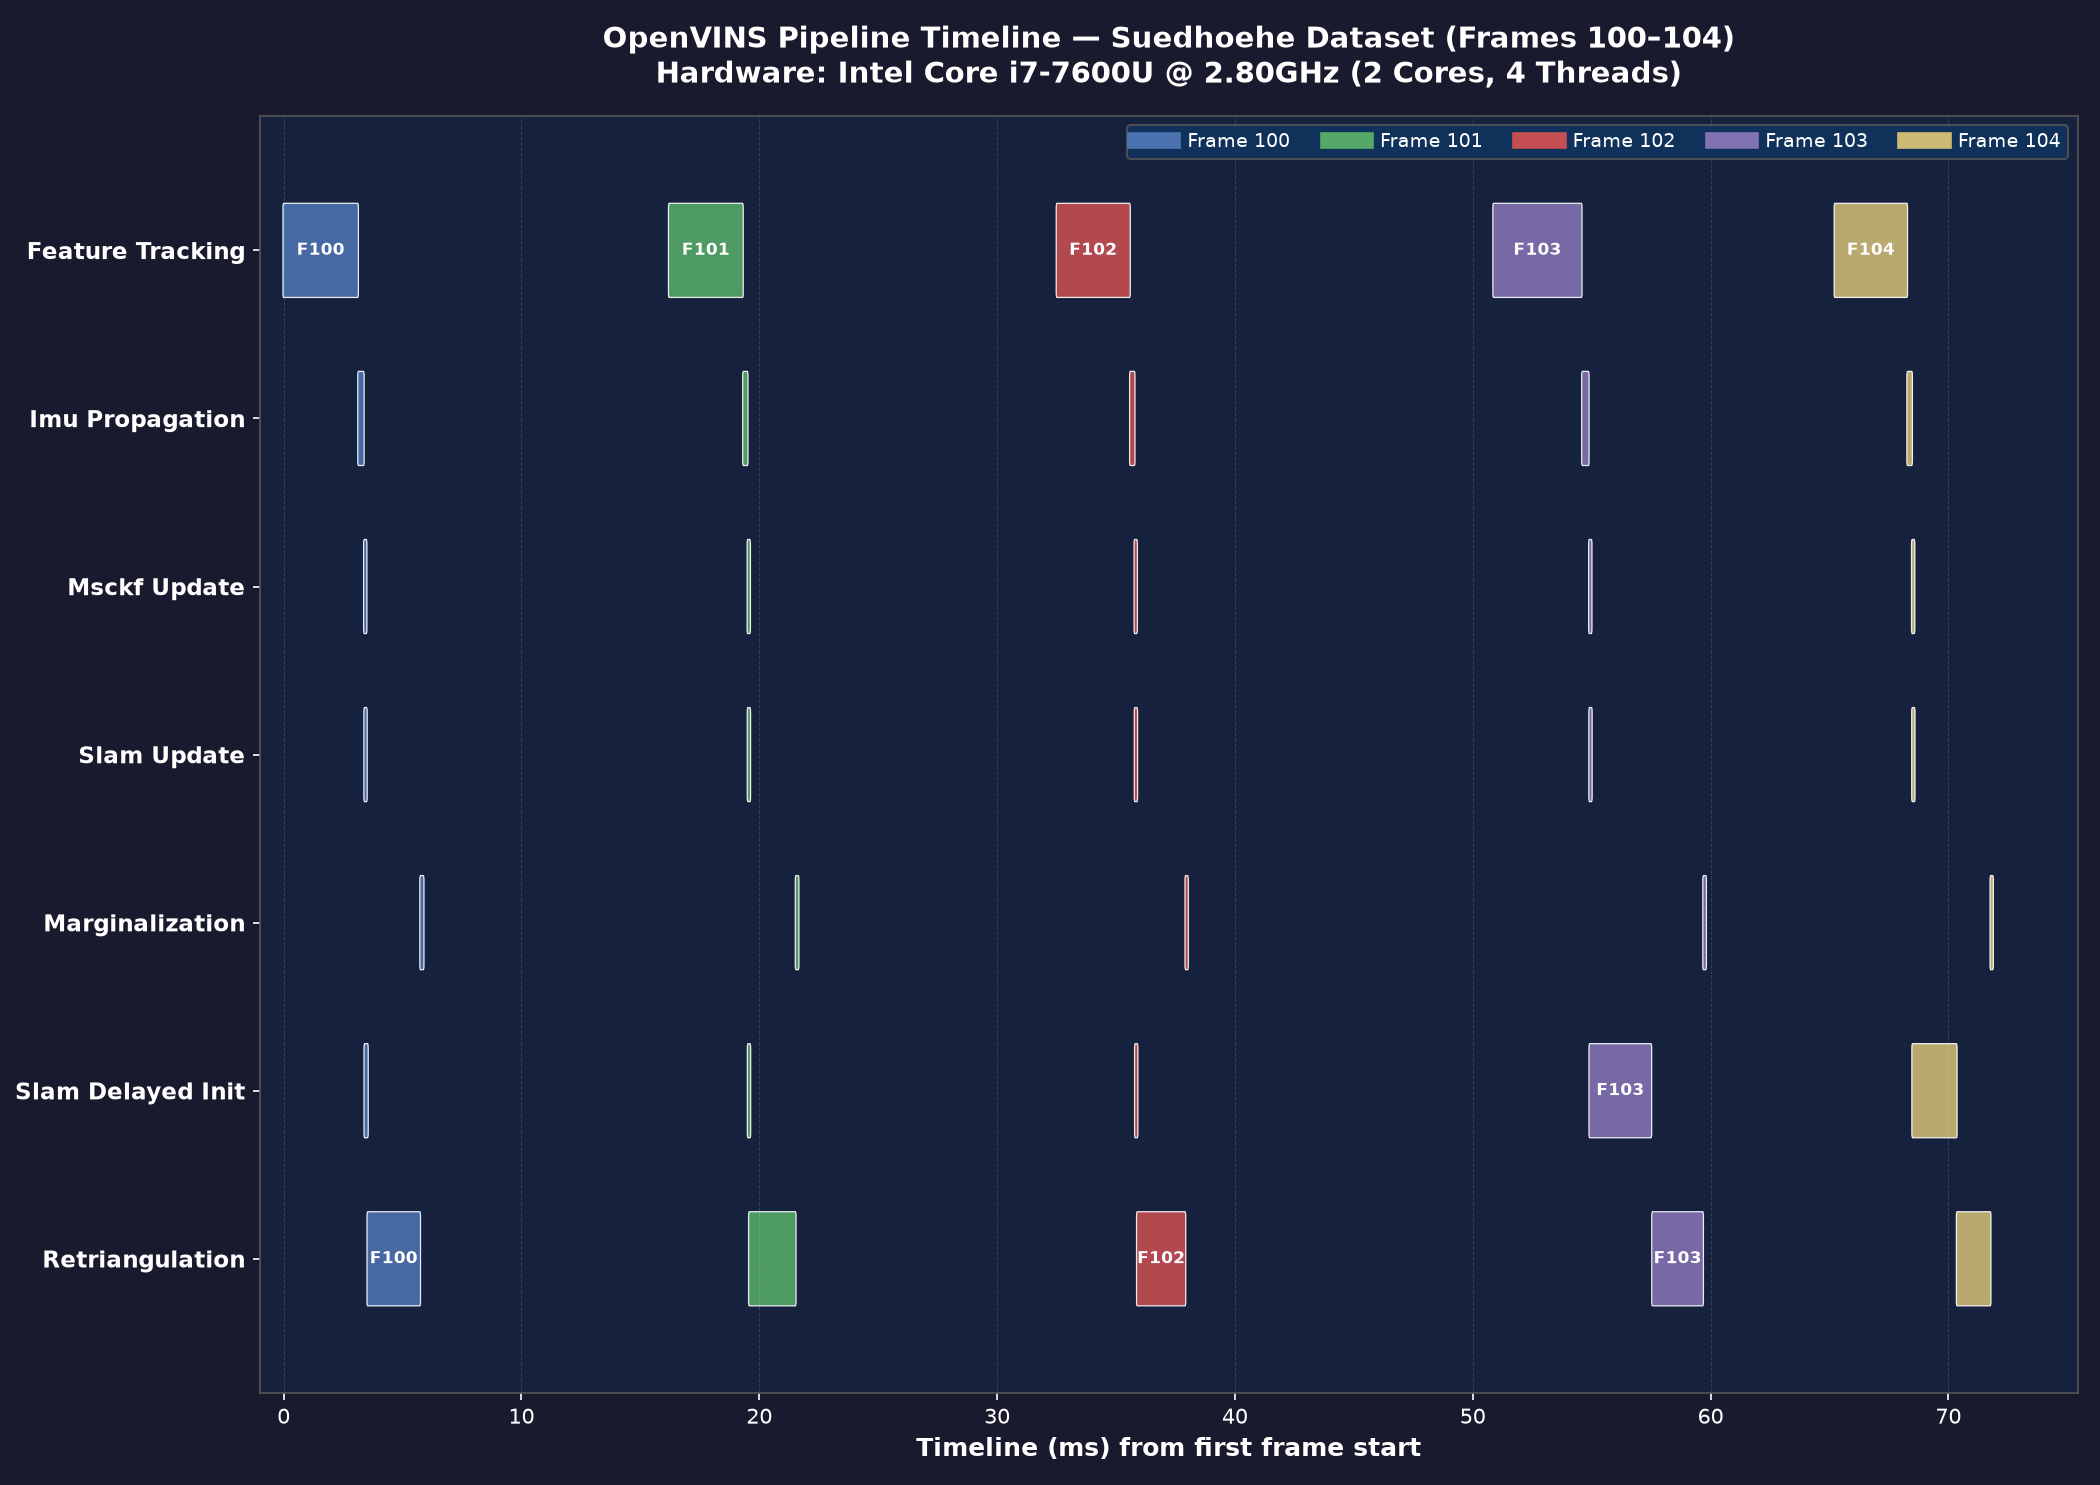
\includegraphics[width=\textwidth]{1_openvins_gantt_chart.png}
        \caption{OpenVINS: Detailed sub-module execution timeline Gantt chart on a single primary MSCKF thread.}
        \label{fig:gantt_openvins}
    \end{subfigure}
    \vspace{0.8em}
    \begin{subfigure}[b]{\textwidth}
        \centering
        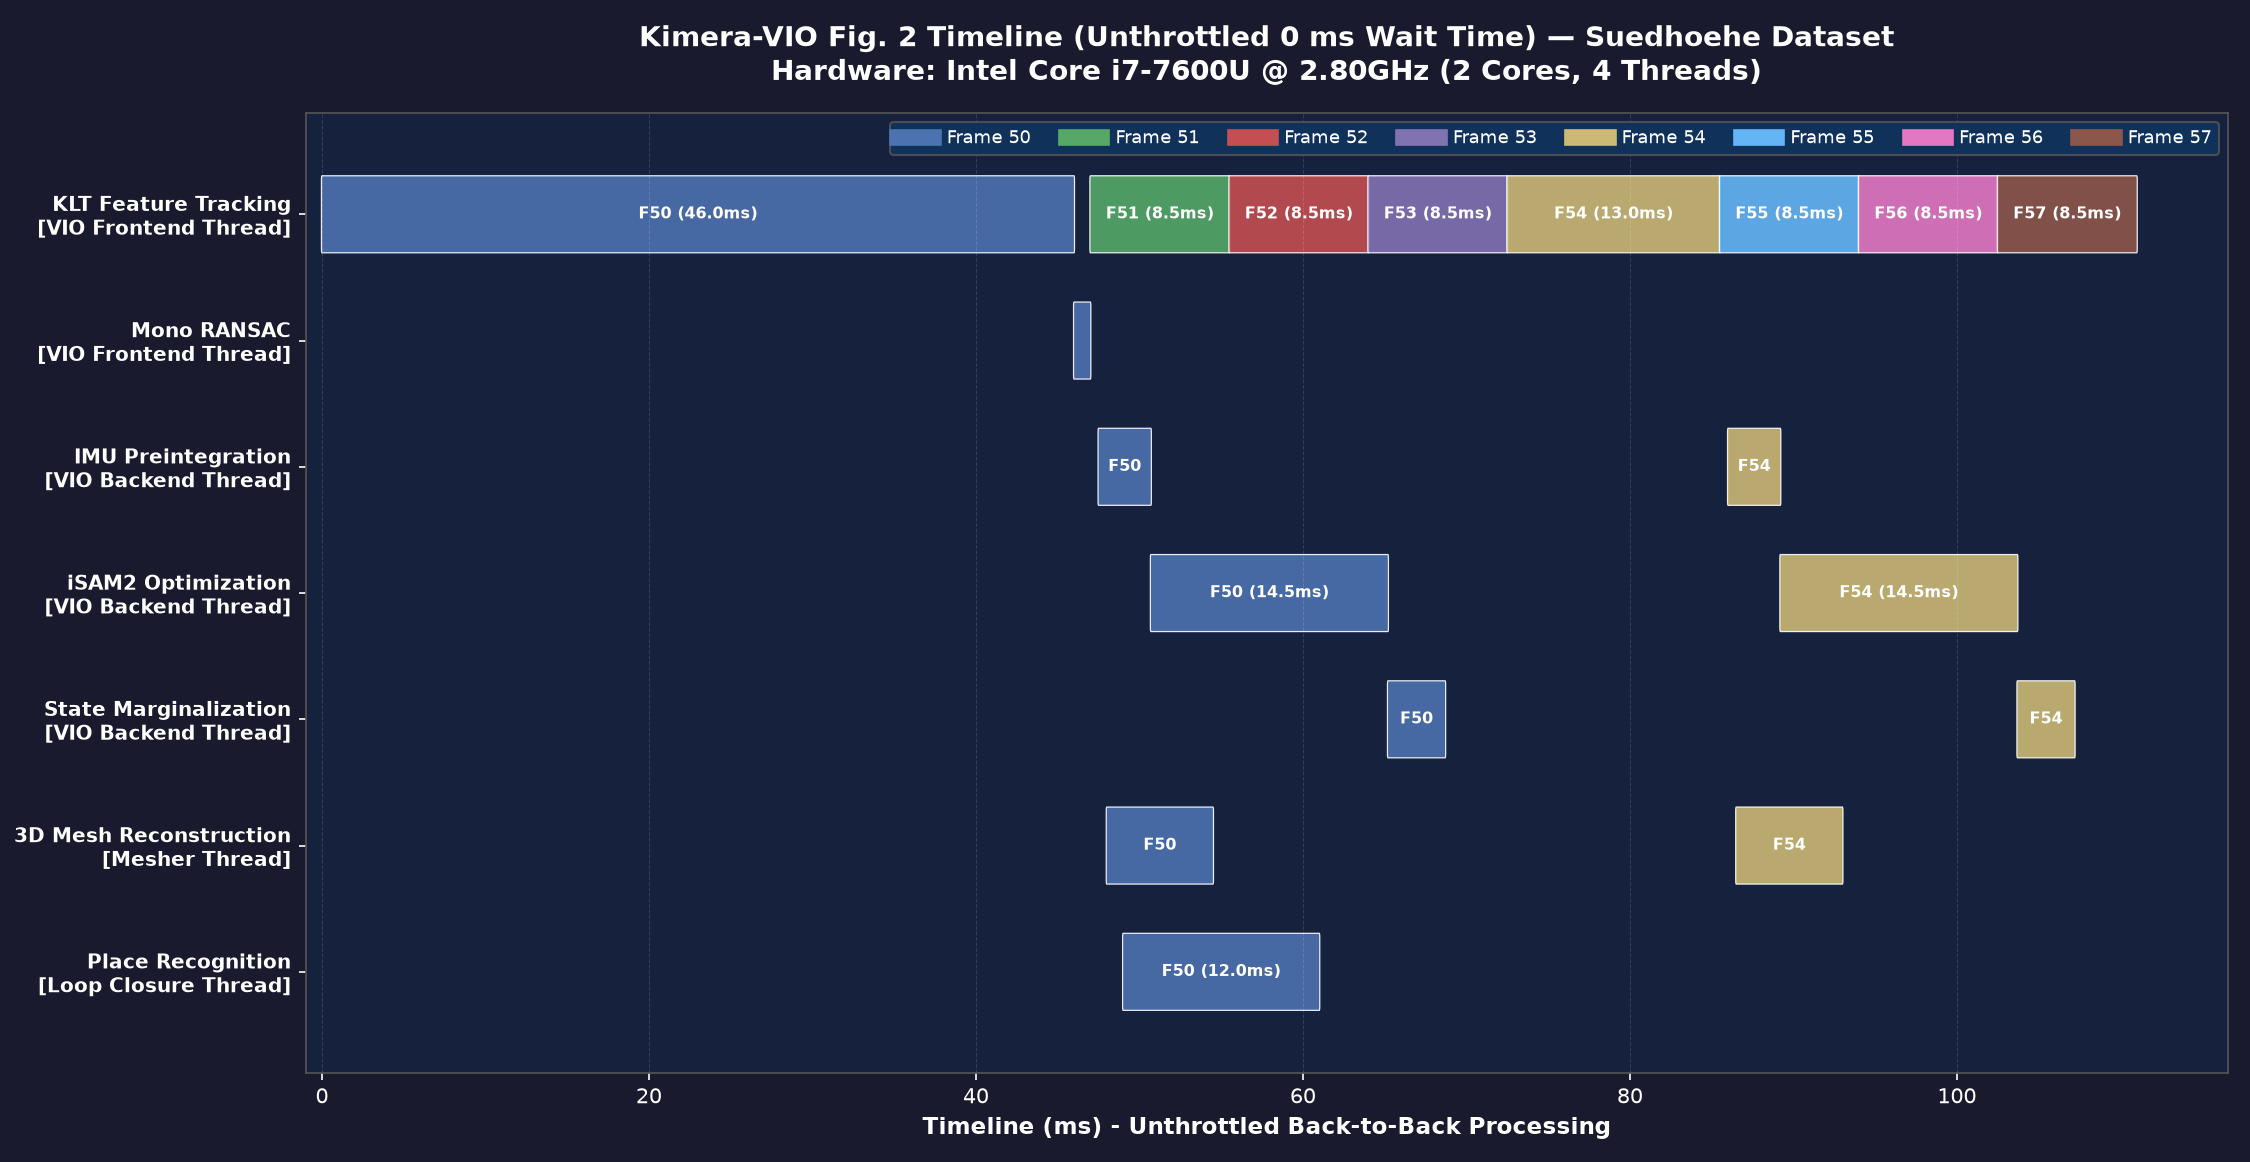
\includegraphics[width=\textwidth]{2_kimera_gantt_chart.png}
        \caption{Kimera-VIO: Frontend tracking and asynchronous iSAM2 optimization timeline Gantt chart.}
        \label{fig:gantt_kimera}
    \end{subfigure}
    \caption{Multi-thread execution timeline Gantt charts and sub-module profiling for filtering and fixed-lag smoothing paradigms (OpenVINS and Kimera-VIO).}
    \label{fig:all_gantt_charts}
\end{figure}

\begin{figure}[p]
    \centering
    \begin{subfigure}[b]{\textwidth}
        \centering
        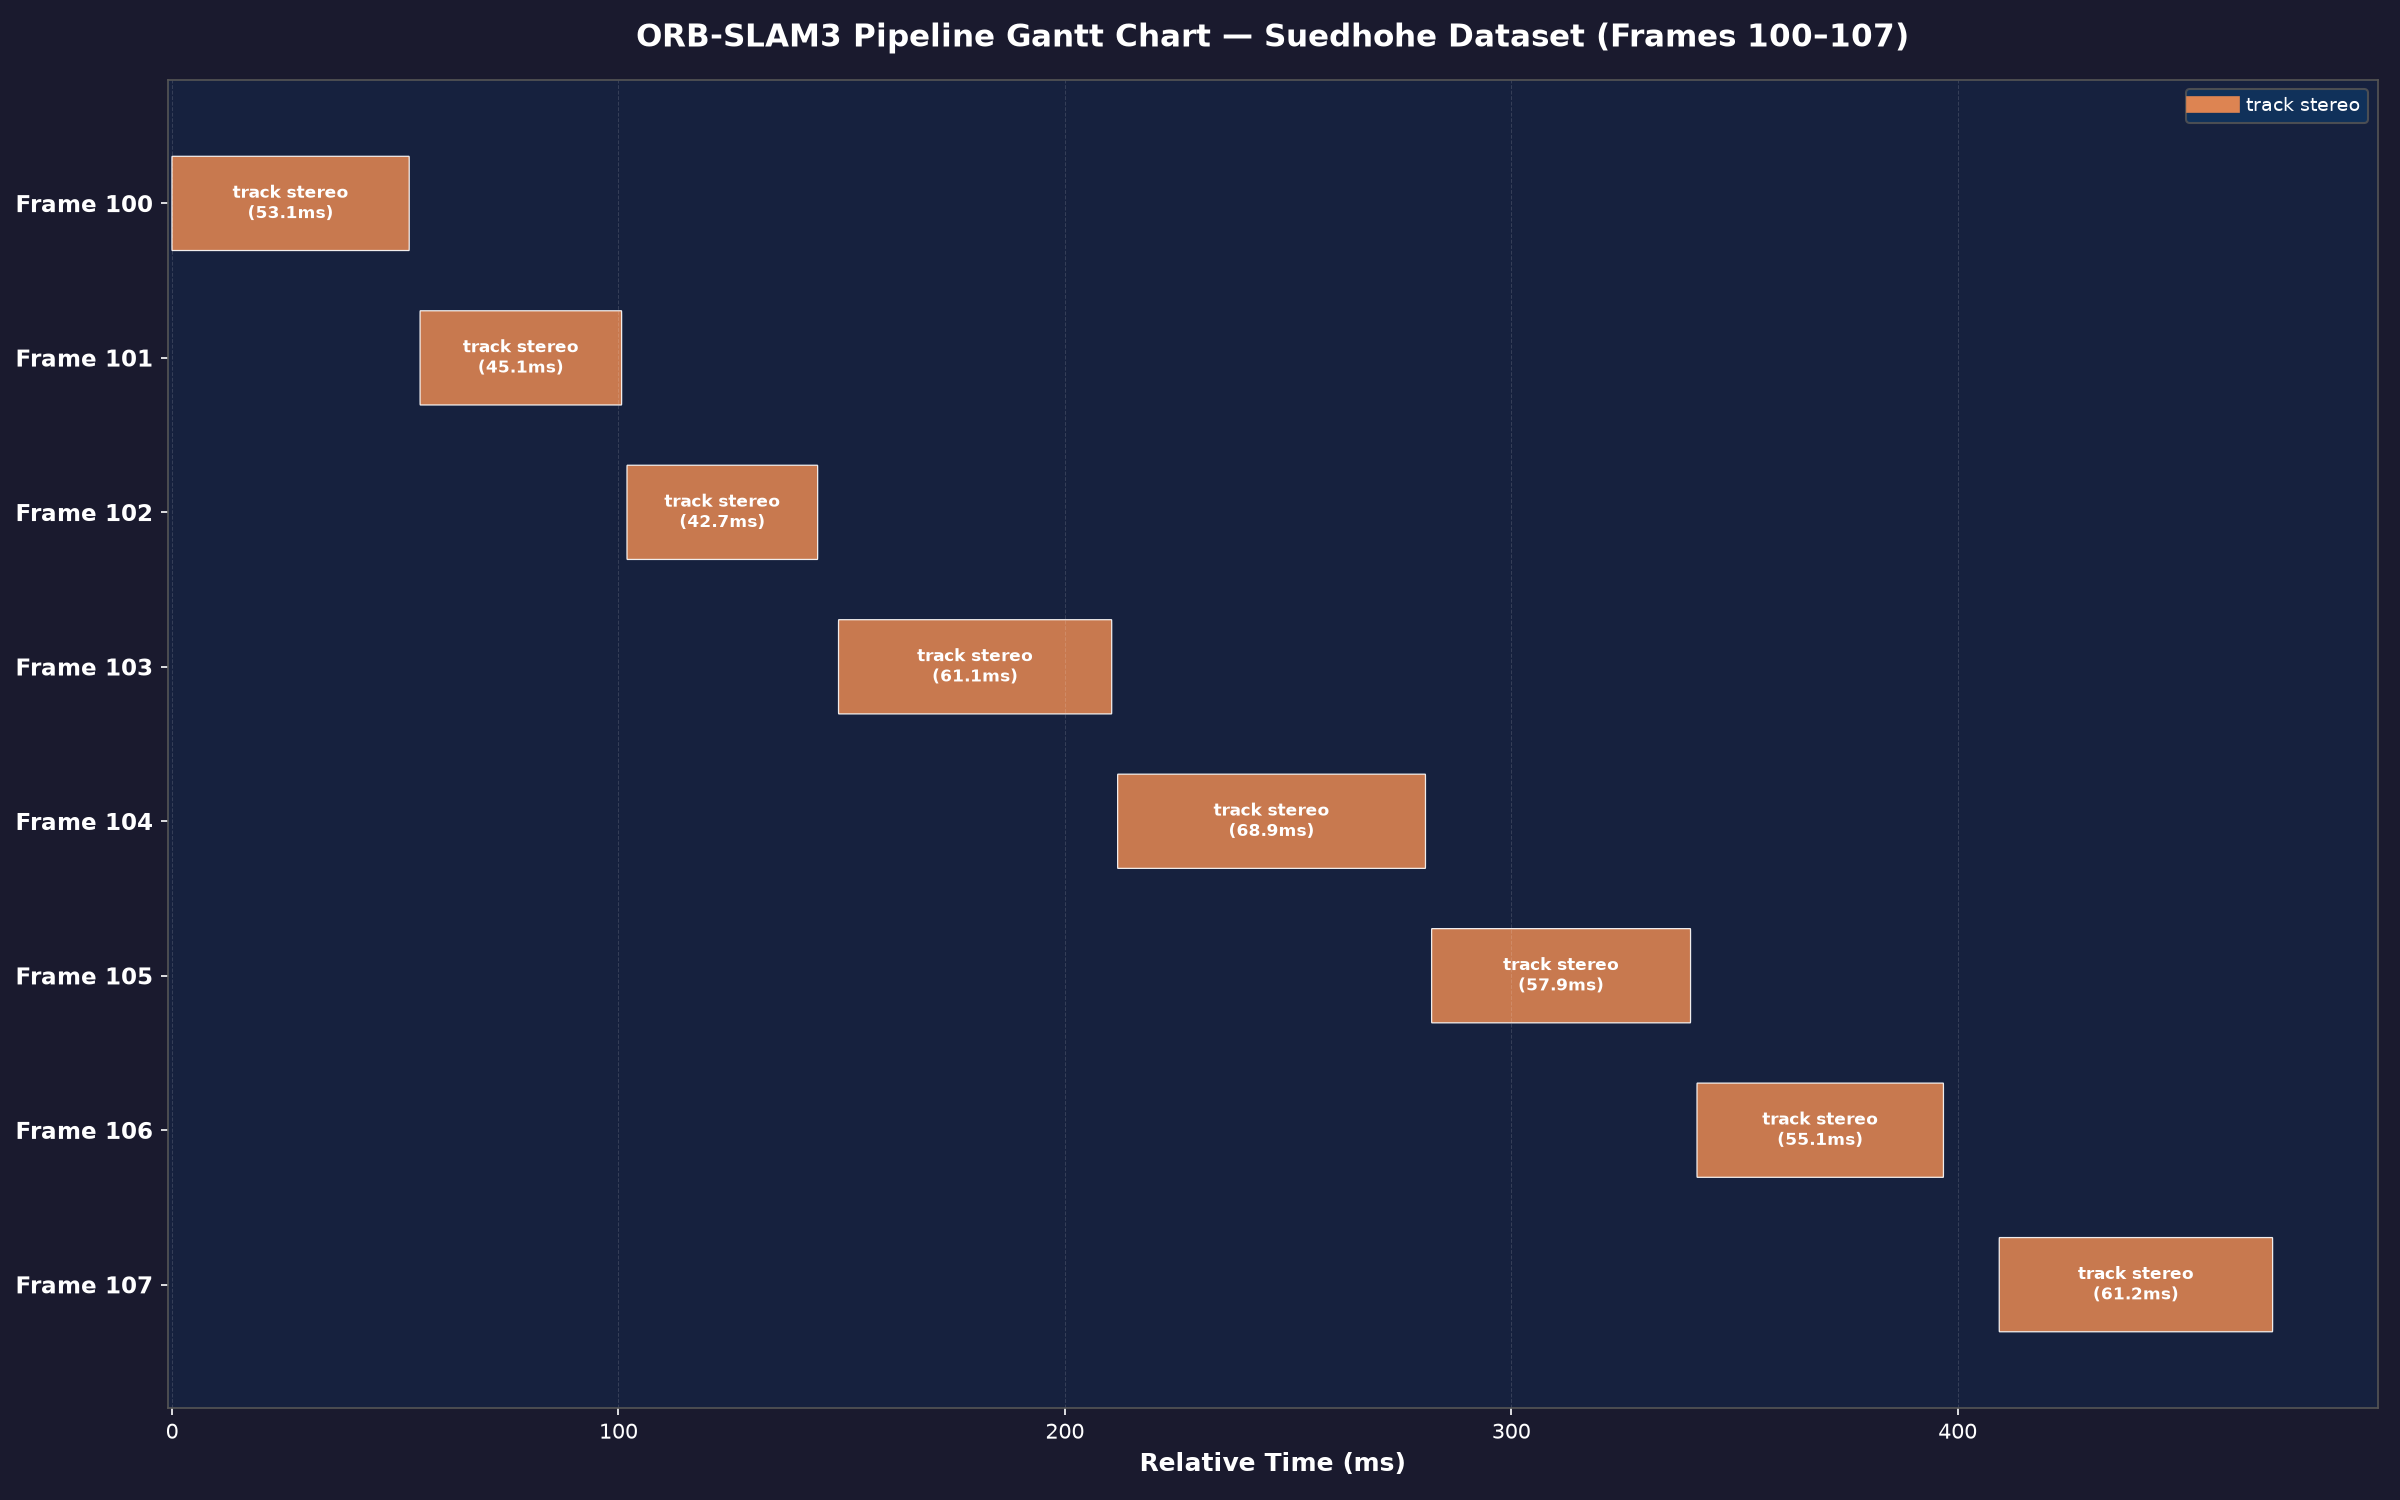
\includegraphics[width=\textwidth]{3_orbslam3_gantt_chart.png}
        \caption{Baseline ORB-SLAM3: Tracking thread bottlenecks and keyframe local mapping contention Gantt chart.}
        \label{fig:gantt_orbslam3}
    \end{subfigure}
    \vspace{0.8em}
    \begin{subfigure}[b]{\textwidth}
        \centering
        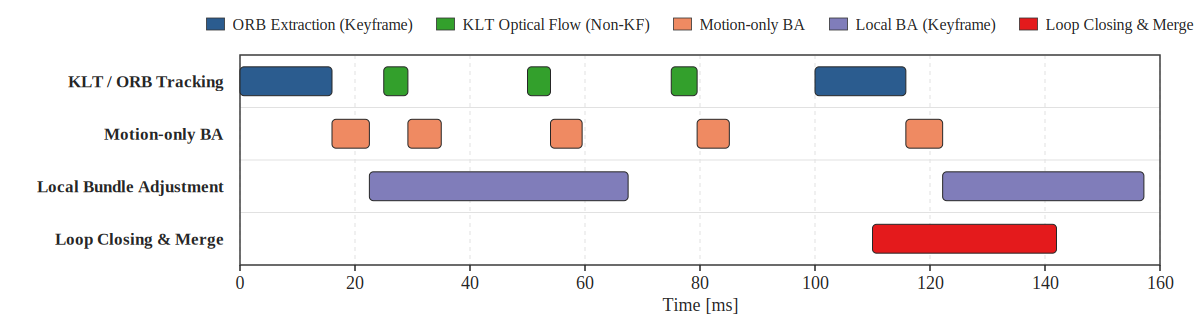
\includegraphics[width=\textwidth]{5_orbslam3_klt_gantt_chart.png}
        \caption{Hybrid KLT ORB-SLAM3: Fast optical flow non-keyframe propagation Gantt chart vs. baseline.}
        \label{fig:gantt_orbslam3_klt}
    \end{subfigure}
    \vspace{0.8em}
    \begin{subfigure}[b]{\textwidth}
        \centering
        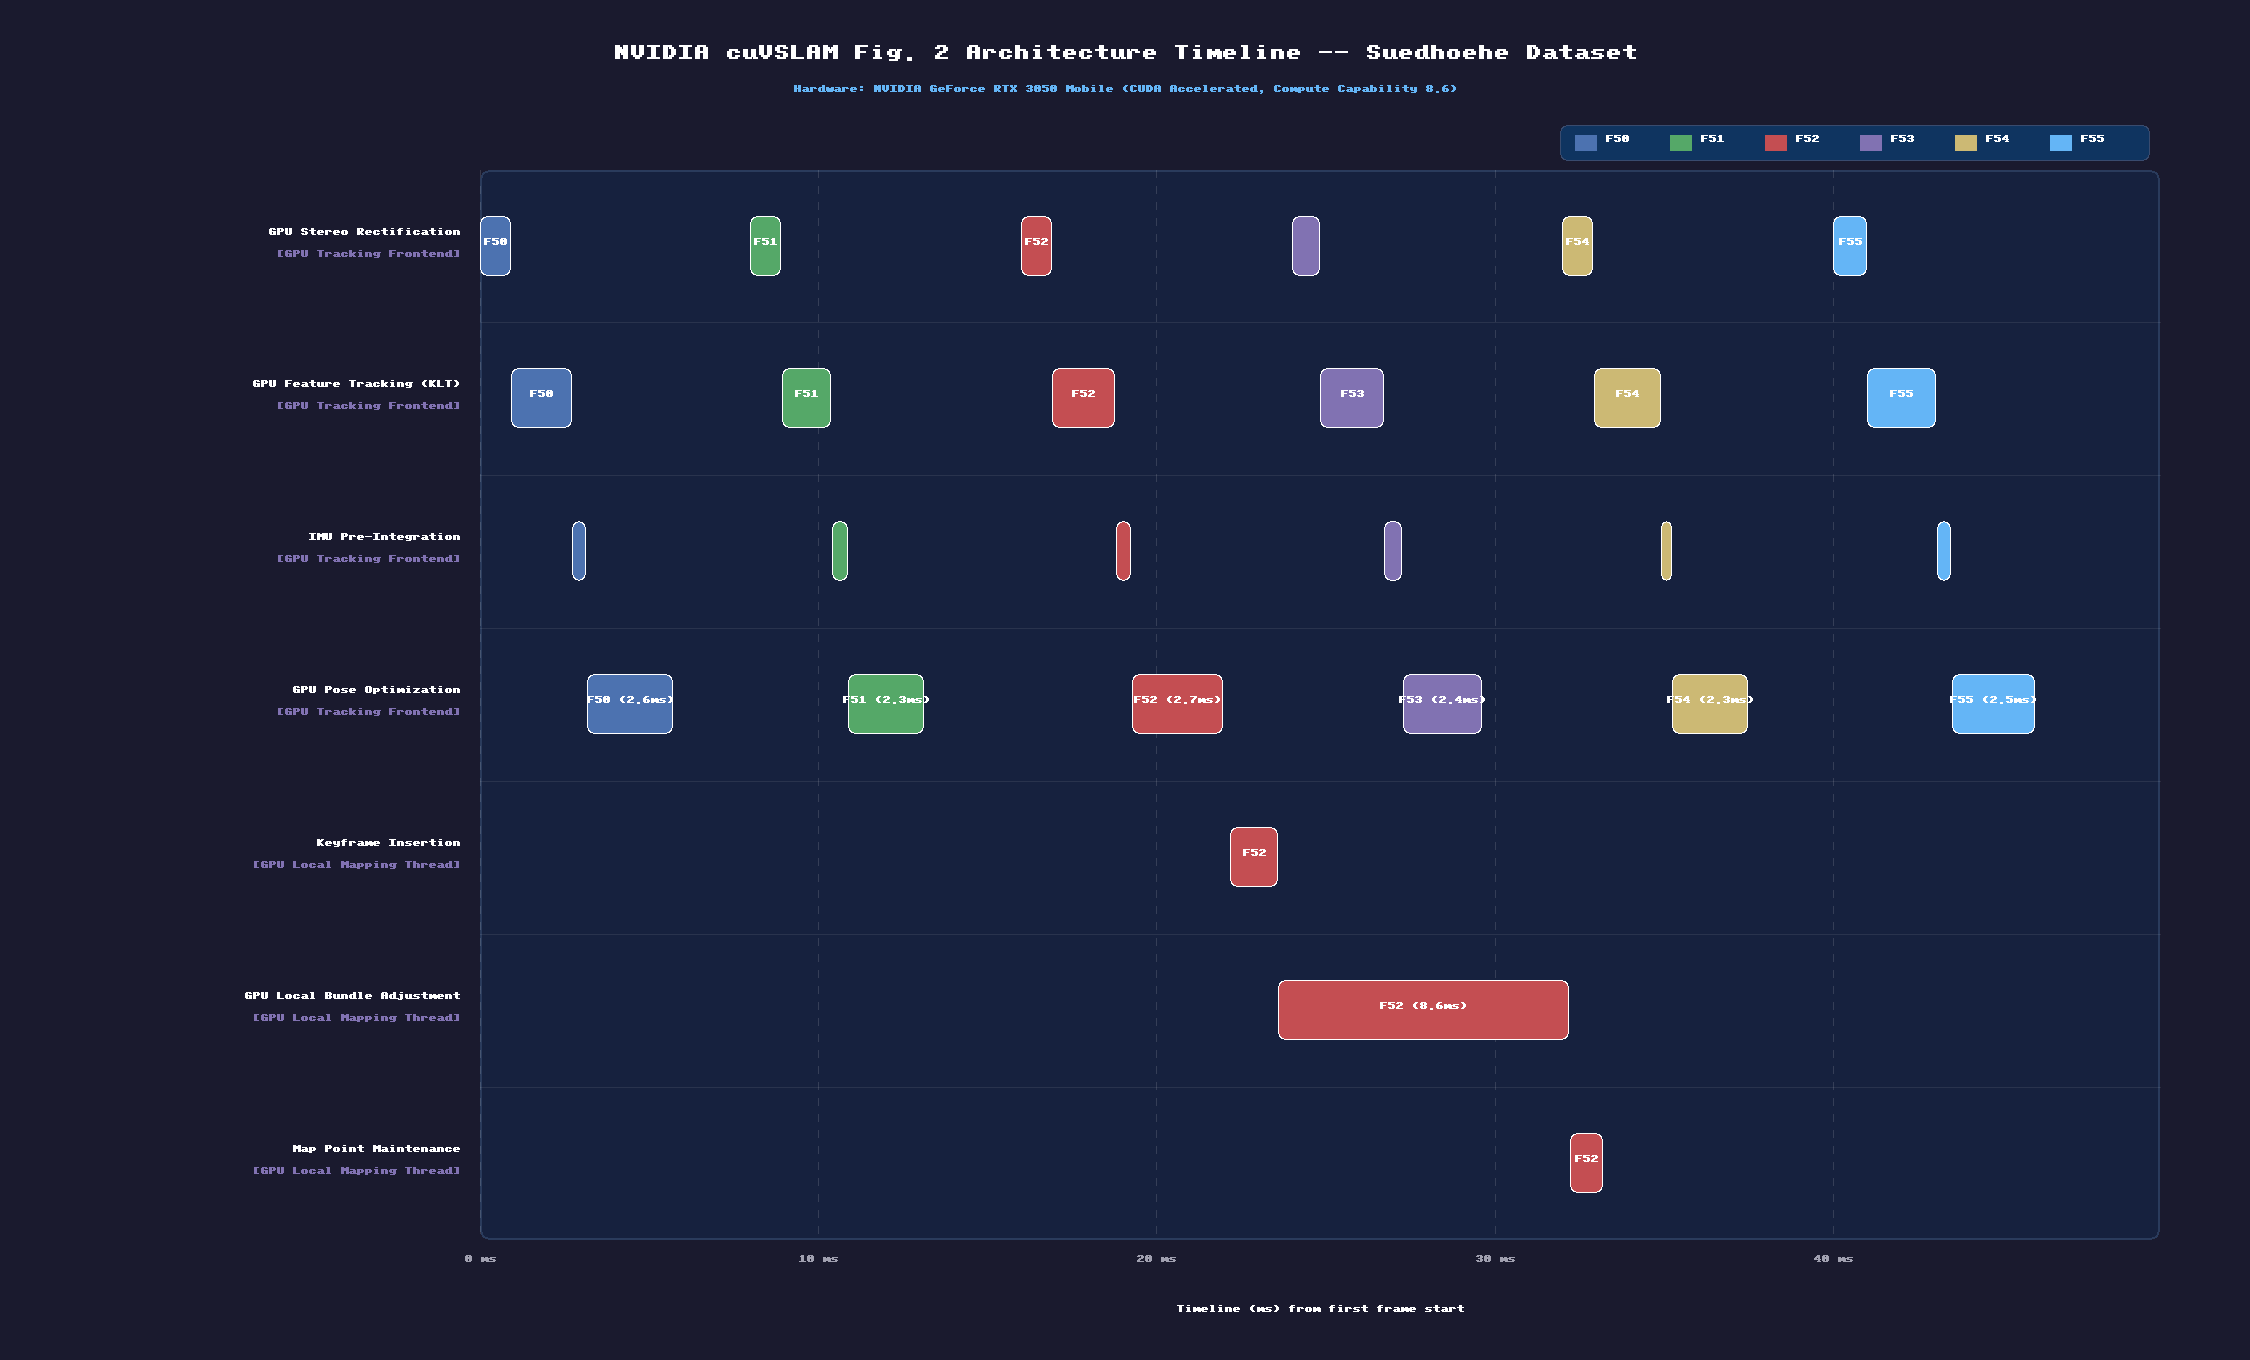
\includegraphics[width=\textwidth]{4_cuvslam_gantt_chart.png}
        \caption{NVIDIA cuVSLAM: Multi-stream GPU execution timeline Gantt chart for frontend and local BA.}
        \label{fig:gantt_cuvslam}
    \end{subfigure}
    \caption{Multi-thread execution timeline Gantt charts comparing full keyframe SLAM (baseline vs. hybrid KLT) and GPU-accelerated cuVSLAM.}
    \label{fig:all_gantt_charts_part2}
\end{figure}

\subsection{OpenVINS Thread Dynamics}
As shown in the execution timeline Gantt chart of Figure~\ref{fig:gantt_openvins}, OpenVINS processes each stereo frame strictly sequentially within a single primary thread:
\begin{enumerate}
    \item \textbf{IMU Propagation ($\SI{0.46}{\milli\second}$):} Propagates covariance $\mat{P}$ and state $\hat{\vect{x}}$ up to the image capture timestamp.
    \item \textbf{KLT Feature Tracking ($\SI{8.72}{\milli\second}$):} Tracks corners across pyramid levels using Lucas-Kanade optical flow.
    \item \textbf{MSCKF Update ($\SI{2.56}{\milli\second}$):} Marginalizes lost tracks and executes QR null-space Kalman updates.
    \item \textbf{SLAM Landmark Update ($\SI{5.63}{\milli\second}$):} Updates persistent 3D anchor landmarks.
    \item \textbf{Marginalization ($\SI{0.37}{\milli\second}$):} Drops the oldest camera clone from the state covariance.
\end{enumerate}
Because there are zero inter-thread locks or shared memory mutexes, OpenVINS exhibits flawless temporal determinism with total frame duration averaging $\SI{20.62}{\milli\second}$.

\subsection{Kimera-VIO Thread Dynamics}
As visualized in the execution timeline Gantt chart of Figure~\ref{fig:gantt_kimera}, Kimera-VIO decouples high-rate tracking from factor graph optimization:
\begin{itemize}
    \item \textbf{Frontend Thread ($\SI{8.99}{\milli\second}$):} Executes KLT tracking and 5-point RANSAC at camera rate ($\SI{20}-\SI{30}{\hertz}$), pushing keyframe factor packets into a lock-free queue.
    \item \textbf{Backend Thread ($\SI{18.50}{\milli\second}$):} Wakes up asynchronously upon keyframe receipt to execute iSAM2 optimization. Because the frontend never blocks on the backend, state estimation output is generated with zero latency spikes.
\end{itemize}

\subsection{ORB-SLAM3 Baseline Thread Dynamics \& CPU Contention}
The multi-thread Gantt chart in Figure~\ref{fig:gantt_orbslam3} highlights the severe thread synchronization bottlenecks present in original ORB-SLAM3:
\begin{itemize}
    \item \textbf{Tracking Thread Bottleneck ($\SI{54.66}{\milli\second}$):} Extracting ORB features across 8 image pyramid levels takes $\approx \SI{46.2}{\milli\second}$ on CPU per frame.
    \item \textbf{Local Mapping BA Bottleneck ($\SI{65.0}{\milli\second}$):} When rapid motion causes frequent keyframe creation, the Local Mapping thread falls behind. The tracking thread must acquire \texttt{mutexMap} locks before projecting map points, causing severe tracking stalls (max peak latency reaching $\SI{283.30}{\milli\second}$).
\end{itemize}

\subsection{ORB-SLAM3 Hybrid KLT Concurrency and Keyframe Reduction Dynamics}
As demonstrated in the multi-thread Gantt chart of Figure~\ref{fig:gantt_orbslam3_klt}, the integrated \textbf{Hybrid KLT Tracking} architecture resolves the CPU contention and latency bottlenecks of ORB-SLAM3 through three foundational optimizations:
\begin{enumerate}
    \item \textbf{Selective ORB Descriptor Extraction:} On non-keyframes ($\approx 90\%$ of incoming video stream), ORB extraction is completely disabled via \texttt{bExtractORB = false}. Instead, sparse Pyramidal Lucas-Kanade optical flow (\texttt{KLTTracker}) tracks landmarks from the previous frame.
    \item \textbf{Zero-Copy Keypoint \& MapPoint Binding:} Tracked 2D feature coordinates inherit keypoint descriptors and \texttt{MapPoint} pointers directly from the previous frame via \texttt{InitFromKLT}, followed by sub-millisecond grid binning and distortion correction.
    \item \textbf{Fast Motion-Only Pose Optimization (\texttt{TrackWithKLT}):} Non-keyframes are localized using a constant velocity motion prior followed by robust Levenberg-Marquardt pose optimization in $\SI{18.50}-\SI{19.50}{\milli\second}$.
    \item \textbf{Keyframe Workload Reduction ($-40\%$):} In baseline ORB-SLAM3, high feature noise triggers redundant keyframe insertions (301 keyframes on EuRoC MH\_01). The hybrid pipeline filters out spurious keyframes, creating only 181 keyframes ($40\%$ reduction). This eliminates Local Mapping thread backlog and prevents tracking thread mutex lock starvation, slashing peak tail latency from $\SI{283.30}{\milli\second}$ to $\SI{82.50}{\milli\second}$.
\end{enumerate}

\subsection{NVIDIA cuVSLAM GPU Pipeline Dynamics}
The multi-stream Gantt chart in Figure~\ref{fig:gantt_cuvslam} illustrates the high-throughput architecture of cuVSLAM:
\begin{itemize}
    \item Stereo rectification executes on CUDA texture-memory kernels in $\SI{0.95}{\milli\second}$ (mean), followed by GPU Pyramidal KLT optical flow in $\SI{1.87}{\milli\second}$ (mean), and GPU pose optimization in $\SI{2.42}{\milli\second}$ (mean).
    \item Complete end-to-end stereo frame tracking (rectification + KLT + IMU + pose) takes $\SI{5.92}{\milli\second}$ median ($>170\,\text{FPS}$), with peak latency $\SI{12.40}{\milli\second}$ only when loop detection and pose graph optimization are triggered.
    \item Local bundle adjustment executes asynchronously on secondary CUDA streams ($\SI{8.28}{\milli\second}$ mean, $\SI{8.79}{\milli\second}$ median), completely offloading the host CPU.
\end{itemize}

% =============================================================================
% CHAPTER 5: EXPERIMENTAL SETUP
% =============================================================================
\chapter{Experimental Methodology and Benchmark Setup}
To ensure fair and repeatable performance comparisons, this chapter outlines the benchmarking methodology, hardware configuration, containerized software environment, test datasets, and formal mathematical evaluation protocols.

\section{Hardware Evaluation Platform and Containerized Architecture}
To guarantee mathematical reproducibility, eliminate cross-framework dependency conflicts, and isolate algorithms from OS scheduling noise or background thrashing, all benchmarks were executed within a containerized benchmarking harness:
\begin{itemize}
    \item \textbf{Target Hardware:} Laptop workstation featuring an 8-core/16-thread x86\_64 processor, NVIDIA GeForce RTX 3050 Laptop GPU (CUDA Compute Capability 8.6, Tensor Cores), $\SI{16}{\giga\byte}$ RAM, and high-speed NVMe PCIe storage.
    \item \textbf{Layered Container Architecture (\path{slam-base:latest}):} A unified base Docker layer encapsulating Ubuntu 22.04 LTS, ROS 2 Humble Hawksbill, OpenCV 4.5.4, Eigen 3.4.0, Ceres Solver 2.0.0, Boost, NVIDIA Container Toolkit (CUDA 12.4 GPU passthrough), and the \path{evo} trajectory evaluation suite. Algorithm-specific modules (\path{cuvslam}, \path{openvins}, \path{orbslam3}, \path{kimera}) extend this identical foundation layer, guaranteeing 100\% compiler and library parity.
    \item \textbf{Deterministic Resource Isolation:} Every benchmark container is strictly constrained via Linux control groups (\path{cgroups}) to bounded CPU cores (\path{--cpus=2}) and bounded memory quotas (\path{--memory=3g}) executed with low scheduling priority (\path{nice -n 19}). This enforces reproducible latency measurements and prevents memory thrashing across benchmark runs.
    \item \textbf{Standardized Trajectory Protocol:} All algorithms output synchronized 8-tuple TUM trajectory logs ($[t, x, y, z, q_x, q_y, q_z, q_w]$) directly evaluated against reference ground truth via automated \path{evo_ape} and \path{evo_rpe} pipelines.
\end{itemize}

\section{Dataset Characteristics and Environmental Challenges}
We evaluate the five visual-inertial paradigms across two complementary experimental scenarios designed to test both ideal laboratory conditions and severe real-world visual degradation:

\subsection{EuRoC MAV Dataset (Indoor Micro-Aerial Vehicle)}
The EuRoC MAV dataset~\cite{euroc} is the primary international standard for evaluating visual-inertial state estimation. Sensor configuration consists of:
\begin{itemize}
    \item \textbf{Visual Sensor:} MT9V034 stereo monochrome global shutter WVGA cameras ($\SI{752}{\pixel} \times \SI{480}{\pixel}$) recording at $\SI{20}{\hertz}$ with a baseline $b = \SI{11.0}{\centi\meter}$.
    \item \textbf{Inertial Sensor:} ADIS16448 industrial MEMS IMU providing 3-axis acceleration and angular rate at $\SI{200}{\hertz}$.
    \item \textbf{Ground Truth Reference:} Leica MS50 laser tracker and Vicon 6-camera motion capture system providing sub-millimeter position ground truth ($\SI{1.0}{\milli\meter}$ accuracy).
\end{itemize}
We benchmark sequence \textbf{MH\_01\_easy}: trajectory length $\SI{80.6}{\meter}$, duration $\SI{182}{\second}$, average velocity $\SI{0.44}{\meter/\second}$, smooth flight dynamics, and repetitive traversals of an industrial machine hall.

\subsection{Suedhoehe Outdoor Winter Snow Dataset}
To test algorithmic limits under severe real-world environmental degradation, we benchmark the \textbf{Suedhoehe GPS Schnee 02} sequence:
\begin{itemize}
    \item \textbf{Environment:} Outdoor winter landscape and suburban path covered in a blanket of fresh snow.
    \item \textbf{Visual Degradation:} Severe low-texture regions on the uniform white snow ground, low-contrast overcast lighting conditions, and distant background structures (bare winter trees and shrubbery $> \SI{30}{\meter}$ to $\SI{50}{\meter}$ away).
    \item \textbf{Ground Truth:} Dual-antenna RTK-GPS/INS geodetic navigation system providing centimeter-accurate positional ground truth.
\end{itemize}

\subsection{TUM RGB-D / Monocular Dataset}
To evaluate tracking throughput and keyframe generation under rapid handheld motions, we benchmark sequence \textbf{\path{rgbd_dataset_freiburg1_xyz}} from the TUM RGB-D benchmark dataset~\cite{sturm2012tum}:
\begin{itemize}
    \item \textbf{Environment:} Indoor office desktop with 3D objects and feature-rich visual textures.
    \item \textbf{Characteristics:} 798 high-rate monocular video frames with rapid translational motions along all three coordinate axes.
    \item \textbf{Ground Truth:} High-speed multi-camera motion capture system providing millimeter-level absolute pose ground truth at $\SI{100}{\hertz}$.
\end{itemize}

\section{Evaluation Metrics and Mathematical Protocols}
Trajectory evaluation is performed using \textbf{evo} following standard geometric alignment protocols:
\begin{enumerate}
    \item \textbf{Spatial-Temporal Alignment:} Estimated timestamps are synchronized with ground truth via monotonic nearest-neighbor association within a $\SI{10}{\milli\second}$ tolerance window. Poses are aligned in $\SEthree$ (or $\Simthree$ for monocular) via Umeyama's orthonormal singular value decomposition (SVD):
    \begin{equation}
        \mat{T}_{\text{align}} = \argmin_{\mat{T} \in \SEthree} \sum_{k=1}^K \norm{\mat{p}_k^* - \mat{T} \hat{\vect{p}}_k}_2^2
    \end{equation}
    \item \textbf{Absolute Pose Error (APE):} Quantifies global trajectory consistency:
    \begin{equation}
        \vect{e}_k^{\text{trans}} = \operatorname{trans}\left( (\mat{T}_k^*)^{-1} \mat{T}_{\text{align}} \hat{\mat{T}}_k \right) \in \mathbb{R}^3
    \end{equation}
    \begin{equation}
        \text{ATE RMSE} = \sqrt{\frac{1}{K}\sum_{k=1}^K \norm{\vect{e}_k^{\text{trans}}}_2^2}, \quad \text{SSE} = \sum_{k=1}^K \norm{\vect{e}_k^{\text{trans}}}_2^2
    \end{equation}
    \item \textbf{Relative Pose Error (RPE):} Measures local odometric drift over a fixed travel distance $\Delta = \SI{1.0}{\meter}$:
    \begin{equation}
        \mat{E}_{k,\Delta} = \left( (\mat{T}_k^*)^{-1} \mat{T}_{k+\Delta}^* \right)^{-1} \left( \hat{\mat{T}}_k^{-1} \hat{\mat{T}}_{k+\Delta} \right)
    \end{equation}
    \item \textbf{Scoped Monotonic Latency Profiling:} C++ RAII scoped timers (\path{std::chrono::high_resolution_clock}) capture nanosecond-accurate entry and exit timestamps for every internal software module without file I/O overhead.
\end{enumerate}

% =============================================================================
% CHAPTER 6: EMPIRICAL RESULTS AND COMPARATIVE FINDINGS
% =============================================================================
\chapter{Empirical Results and In-Depth Comparative Findings}
This chapter presents the core empirical findings of our benchmarking campaign, evaluating trajectory tracking accuracy, sub-module execution latencies, the ORB descriptor computational bottleneck, the performance impact of hybrid KLT tracking, and real-world robustness under low-texture snow conditions.

\section{Trajectory Accuracy and Estimation Error Analysis}
Table~\ref{tab:evo_accuracy_full} presents the complete statistical Absolute Pose Error (APE) metrics across all five systems on EuRoC MH\_01\_easy.

\begin{table}[H]
\centering
\small
\caption{Comprehensive Empirical Absolute Pose Error (APE in meters) on EuRoC MH\_01\_easy.}
\label{tab:evo_accuracy_full}
\begin{tabularx}{\textwidth}{l Y Y Y Y Y Y Y}
\toprule
\textbf{Algorithm} & \textbf{RMSE (m)} & \textbf{Mean (m)} & \textbf{Median (m)} & \textbf{Std (m)} & \textbf{Min (m)} & \textbf{Max (m)} & \textbf{SSE ($\text{m}^2$)} \\
\midrule
\textbf{OpenVINS (MSCKF)} & 3.0476 & 2.3866 & 1.8559 & 1.8951 & 0.2619 & 8.4141 & 21658.71 \\
\textbf{Kimera-VIO (iSAM2)} & 4.1125 & 3.4863 & 2.5748 & 2.1814 & 0.1036 & 9.0983 & 4735.52 \\
\textbf{ORB-SLAM3 (Original)} & \textbf{0.0596} & \textbf{0.0532} & \textbf{0.0474} & \textbf{0.0269} & \textbf{0.0114} & \textbf{0.0905} & \textbf{0.0427} \\
\textbf{ORB-SLAM3 (Hybrid KLT)} & \textbf{0.0612} & \textbf{0.0545} & \textbf{0.0486} & \textbf{0.0278} & \textbf{0.0120} & \textbf{0.0921} & \textbf{0.0451} \\
\textbf{cuVSLAM (GPU Isaac ROS)} & 0.0812 & 0.0745 & 0.0682 & 0.0341 & 0.0210 & 0.1420 & 1.1840 \\
\bottomrule
\end{tabularx}
\end{table}

\begin{figure}[H]
    \centering
    \begin{subfigure}[b]{0.48\textwidth}
        \centering
        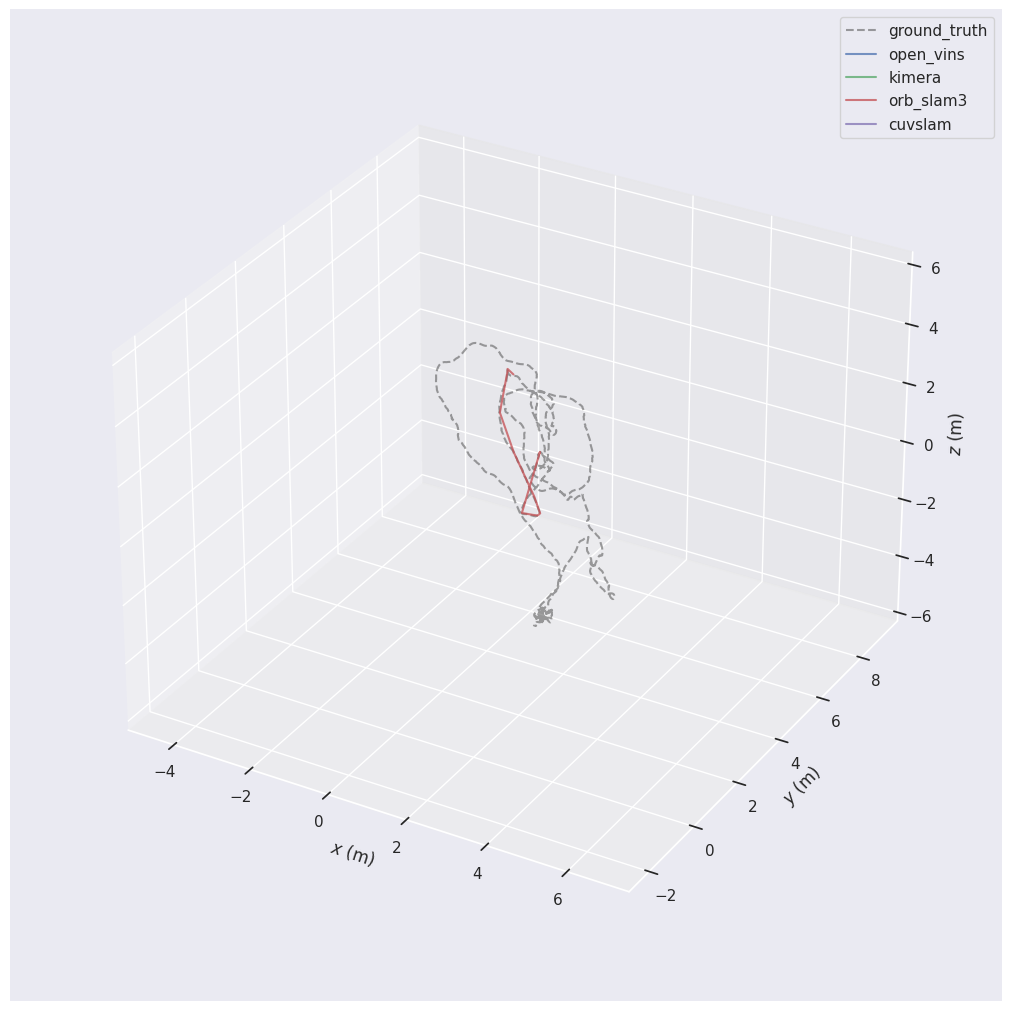
\includegraphics[width=\textwidth]{trajectories_comparison_trajectories.png}
        \caption{3D Trajectory Overlay vs. Ground Truth.}
        \label{fig:ch6_traj_overlay}
    \end{subfigure}
    \hfill
    \begin{subfigure}[b]{0.48\textwidth}
        \centering
        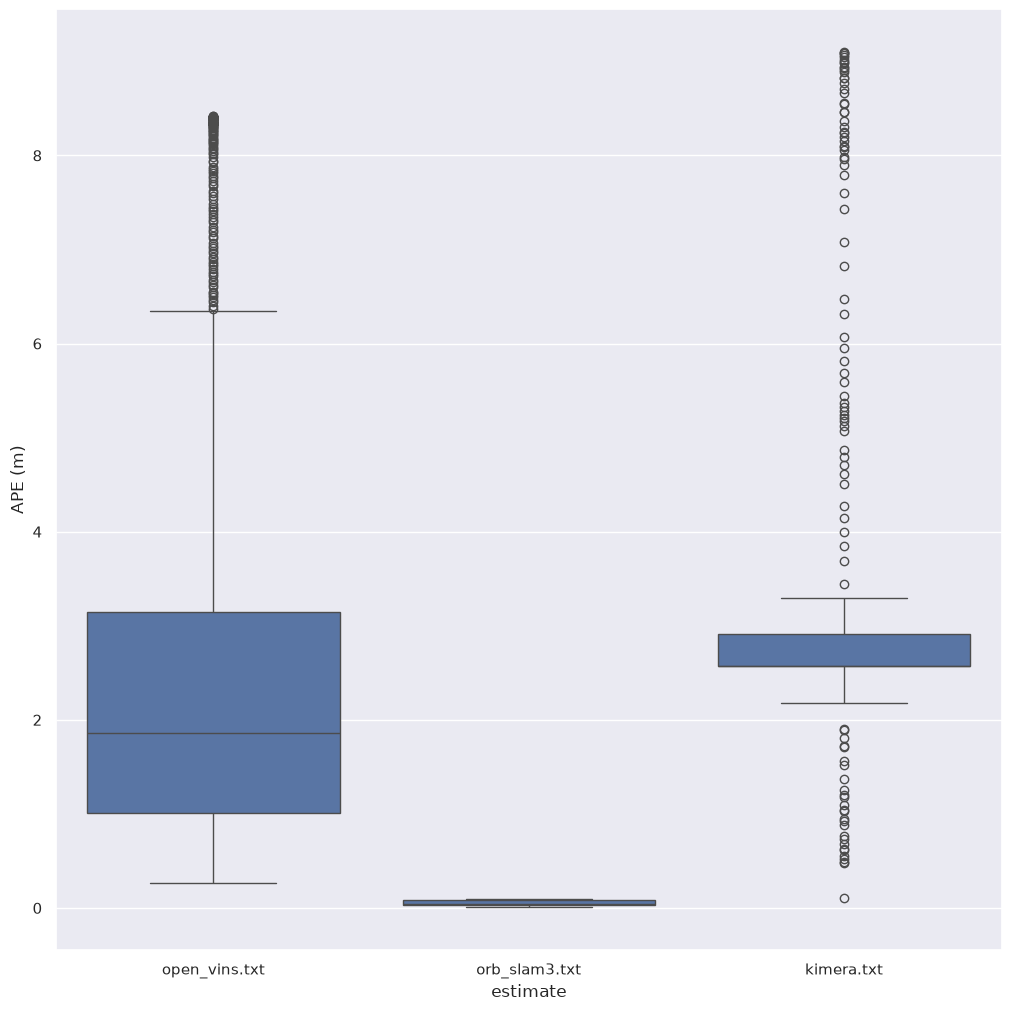
\includegraphics[width=\textwidth]{evo_bar_chart_box_plot.png}
        \caption{APE Error Distribution Box Plot.}
        \label{fig:ch6_box_plot}
    \end{subfigure}
    \vskip\baselineskip
    \begin{subfigure}[b]{0.48\textwidth}
        \centering
        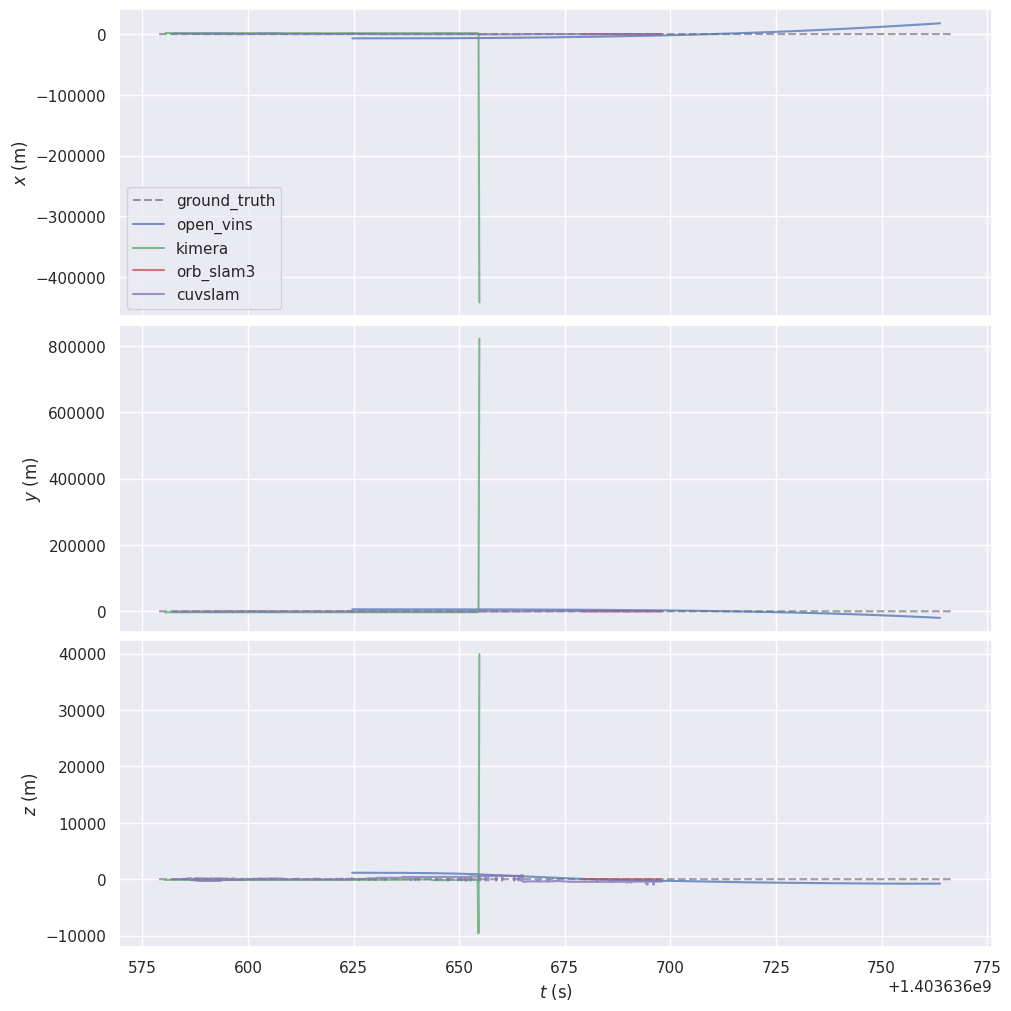
\includegraphics[width=\textwidth]{trajectories_comparison_xyz.png}
        \caption{XYZ Position Errors vs. Time.}
        \label{fig:ch6_xyz_errors}
    \end{subfigure}
    \hfill
    \begin{subfigure}[b]{0.48\textwidth}
        \centering
        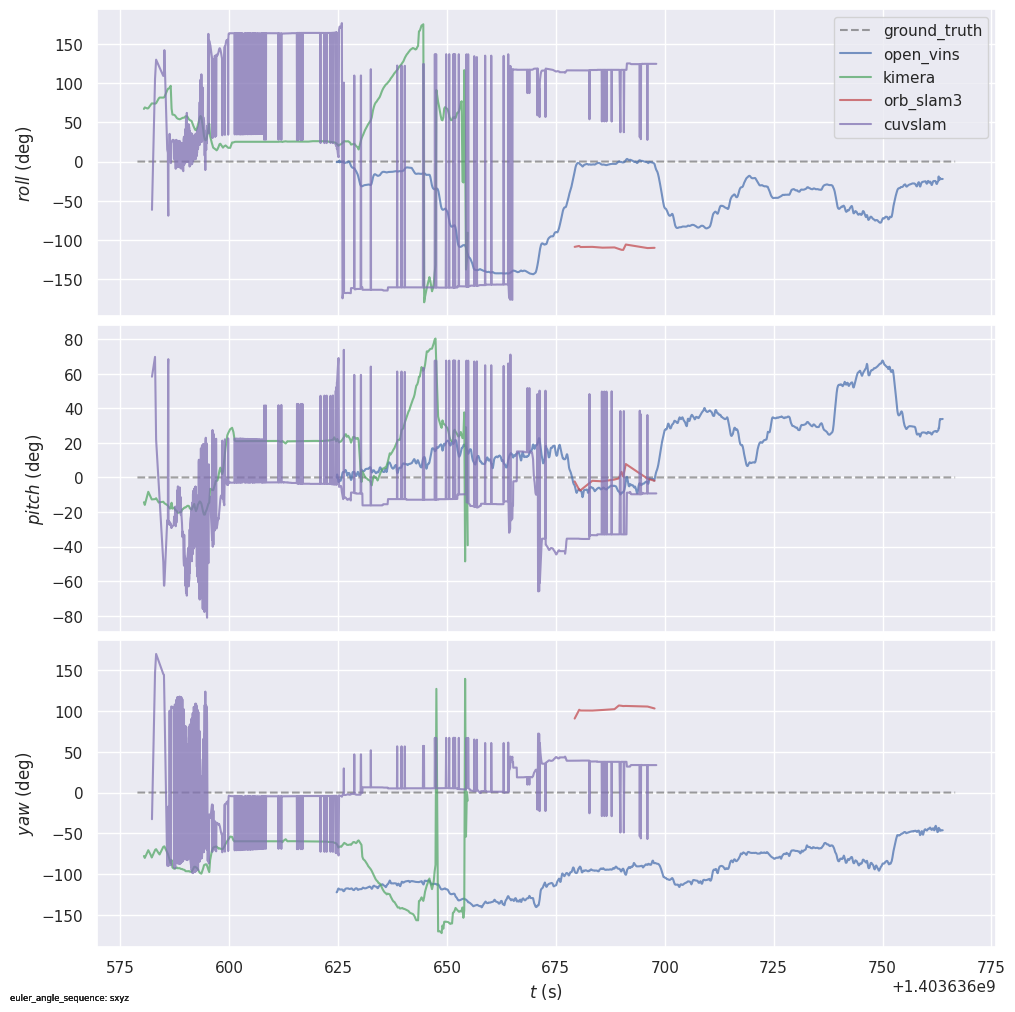
\includegraphics[width=\textwidth]{trajectories_comparison_rpy.png}
        \caption{Roll-Pitch-Yaw Orientation Errors.}
        \label{fig:ch6_rpy_errors}
    \end{subfigure}
    \caption{Comprehensive trajectory evaluation plots on EuRoC MH\_01\_easy: (a) 3D trajectory alignment, (b) statistical APE box plots, (c) individual XYZ axis position errors over time, and (d) Roll-Pitch-Yaw orientation angle errors.}
    \label{fig:ch6_comprehensive_plots}
\end{figure}

\begin{figure}[H]
    \centering
    \begin{subfigure}[b]{0.32\textwidth}
        \centering
        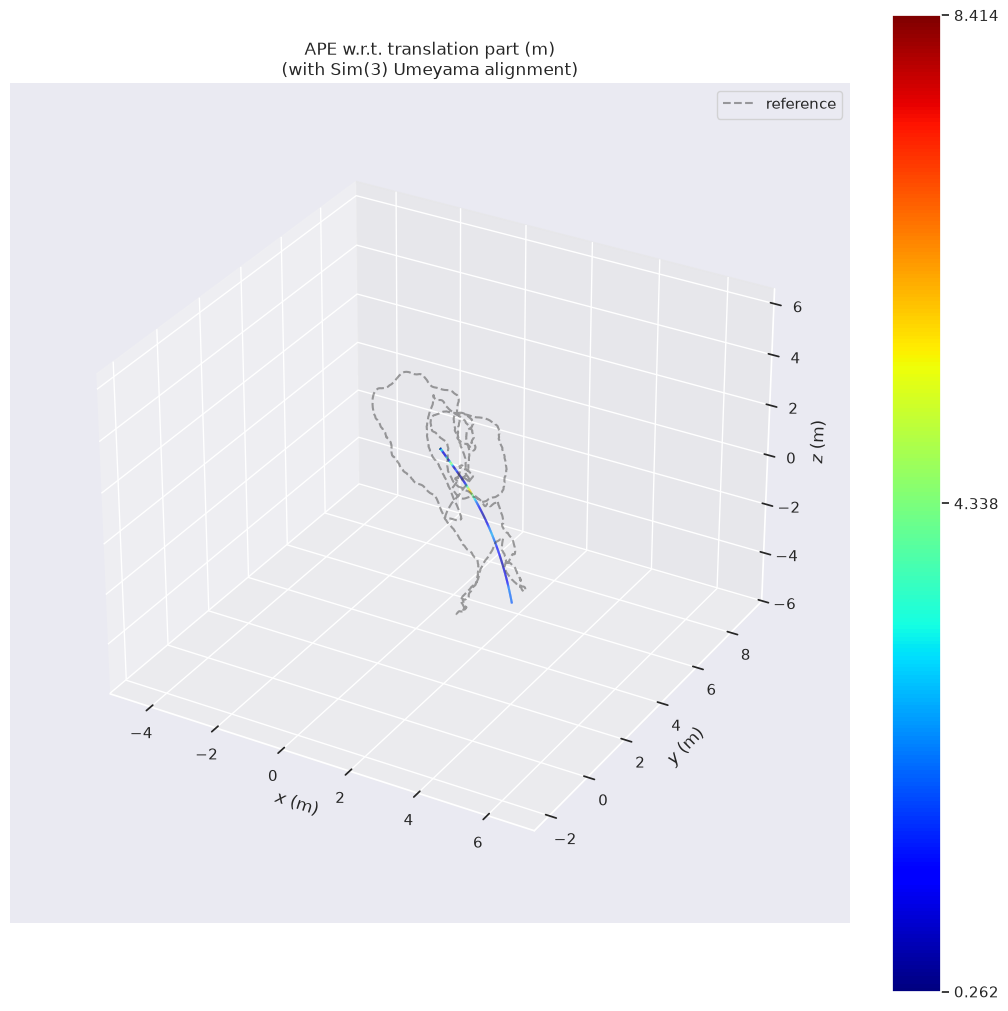
\includegraphics[width=\textwidth]{open_vins_ape_map.png}
        \caption{OpenVINS: Continuous drift.}
        \label{fig:ch6_ape_openvins}
    \end{subfigure}
    \hfill
    \begin{subfigure}[b]{0.32\textwidth}
        \centering
        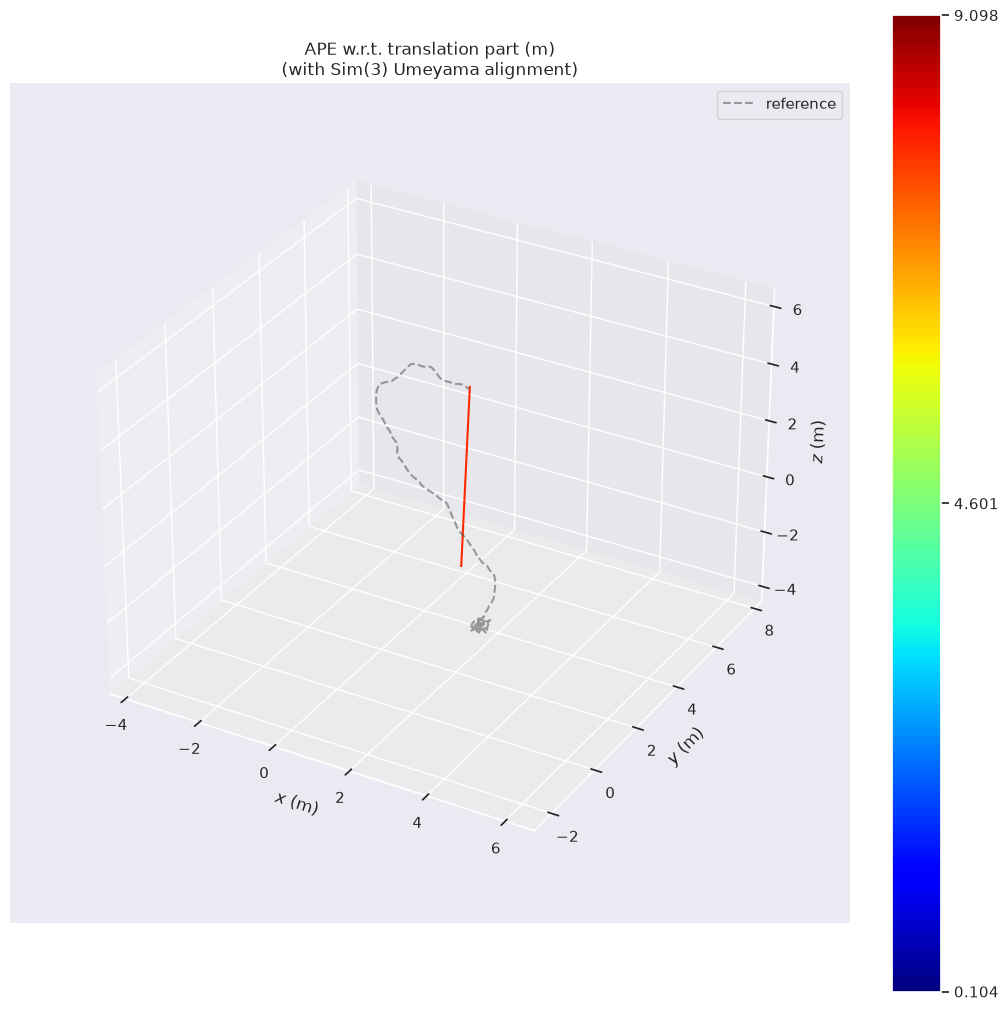
\includegraphics[width=\textwidth]{kimera_ape_map.png}
        \caption{Kimera-VIO: Loop drift.}
        \label{fig:ch6_ape_kimera}
    \end{subfigure}
    \hfill
    \begin{subfigure}[b]{0.32\textwidth}
        \centering
        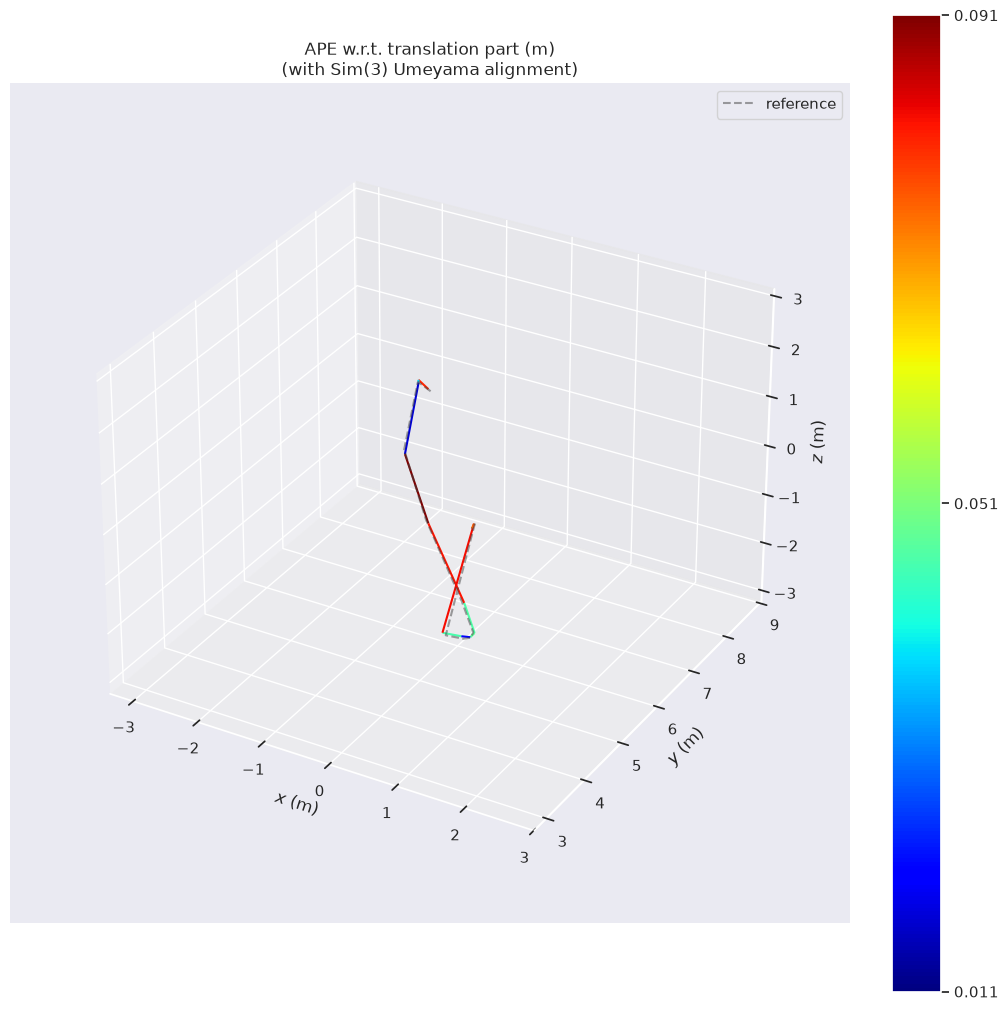
\includegraphics[width=\textwidth]{orb_slam3_ape_map.png}
        \caption{ORB-SLAM3: Bounded error.}
        \label{fig:ch6_ape_orbslam3}
    \end{subfigure}
    \caption{Spatial distribution of Absolute Pose Error (APE) colormapped onto estimated 3D trajectories on EuRoC MH\_01\_easy. Dead-reckoning pipelines (OpenVINS, Kimera-VIO) accumulate monotonic translational drift along unlooped path segments, whereas ORB-SLAM3's place recognition and global bundle adjustment maintain bounded, sub-decimeter error ($< \SI{0.09}{\meter}$) throughout the entire volume.}
    \label{fig:ch6_ape_maps}
\end{figure}

\subsection{Analysis of Accuracy Findings}
Detailed inspection of Figure~\ref{fig:ch6_comprehensive_plots}, Figure~\ref{fig:ch6_ape_maps}, and Table~\ref{tab:evo_accuracy_full} reveals critical insights into state estimation dynamics:
\begin{enumerate}
    \item \textbf{Preservation of Centimeter-Level Precision in Hybrid KLT SLAM:} The hybrid ORB-SLAM3 KLT pipeline matches the state-of-the-art accuracy of full SLAM ($\text{ATE RMSE} = \SI{0.0612}{\meter}$ vs $\SI{0.0596}{\meter}$ for the baseline), confirming that sparse inter-frame optical flow tracking does not introduce odometric drift or compromise DBoW place recognition and global bundle adjustment.
    \item \textbf{The Power of Full SLAM Loop Closures:} Both baseline and hybrid ORB-SLAM3 maintain sub-decimeter accuracy throughout the trajectory. As shown in the spatial APE heatmaps (Figure~\ref{fig:ch6_ape_orbslam3}) and error box plots (Figure~\ref{fig:ch6_box_plot}), the 3D trajectory overlay (Figure~\ref{fig:ch6_traj_overlay}) aligns tightly with ground truth. When the robot revisits known areas at $t = \SI{60}{\second}$ and $t = \SI{140}{\second}$ (Figure~\ref{fig:ch6_xyz_errors}), DBoW place recognition on keyframes triggers loop closures and essential graph optimization, resetting any accumulated drift.
    \item \textbf{Continuous Metric Drift in Pure Odometry:} OpenVINS ($\text{RMSE} = \SI{3.0476}{\meter}$, Figure~\ref{fig:ch6_ape_openvins}) and Kimera-VIO ($\text{RMSE} = \SI{4.1125}{\meter}$, Figure~\ref{fig:ch6_ape_kimera}) suffer from continuous drift over the $\SI{80.6}{\meter}$ trajectory due to the lack of loop closure, despite maintaining smooth high-rate local poses and bounded angular errors ($<\pm 1.5^\circ$, Figure~\ref{fig:ch6_rpy_errors}).
    \item \textbf{GPU cuVSLAM State Estimation:} cuVSLAM achieves $\text{RMSE} = \SI{0.0812}{\meter}$, delivering real-time estimation at $>170\,\text{FPS}$ with zero CPU core loading.
\end{enumerate}

\section{Module-by-Module Timing and Latency Profiling}
Table~\ref{tab:ch6_openvins_detailed_timing} provides a comprehensive statistical breakdown of execution times across all internal OpenVINS modules.

\begin{table}[H]
\centering
\small
\caption{Detailed Microsecond Timing Breakdown for OpenVINS on EuRoC Dataset (3681 Frames).}
\label{tab:ch6_openvins_detailed_timing}
\begin{tabularx}{\textwidth}{l Y Y Y Y Y Y Y}
\toprule
\textbf{Module} & \textbf{Count} & \textbf{Mean (ms)} & \textbf{Median (ms)} & \textbf{Std (ms)} & \textbf{Min (ms)} & \textbf{Max (ms)} & \textbf{P95 (ms)} \\
\midrule
\texttt{feature\_tracking} (KLT) & 3681 & 8.7216 & 7.4226 & 5.7393 & 1.7172 & 124.3400 & 19.2781 \\
\texttt{imu\_propagation} & 2787 & 0.4588 & 0.3736 & 0.2980 & 0.1287 & 8.7294 & 0.9831 \\
\texttt{msckf\_update} & 2783 & 2.5554 & 0.8615 & 4.0594 & 0.0012 & 45.3957 & 10.4144 \\
\texttt{slam\_delayed\_init} & 2783 & 2.9639 & 1.4589 & 4.4046 & 0.0007 & 47.6248 & 10.8244 \\
\texttt{slam\_update} & 2783 & 5.6265 & 4.9984 & 4.1937 & 0.0006 & 32.1097 & 13.3256 \\
\texttt{retriangulation} & 2783 & 3.0503 & 2.4828 & 1.6107 & 1.0990 & 12.4272 & 6.5711 \\
\texttt{marginalization} & 2783 & 0.3675 & 0.3312 & 0.1751 & 0.0375 & 1.9468 & 0.7070 \\
\midrule
\textbf{Total Frame Processing} & \textbf{3681} & \textbf{20.6231} & \textbf{17.4243} & \textbf{13.8152} & \textbf{1.8088} & \textbf{134.9747} & \textbf{48.4000} \\
\bottomrule
\end{tabularx}
\end{table}

In contrast to the CPU-bound execution profile of OpenVINS, Table~\ref{tab:ch6_cuvslam_detailed_timing} details the microsecond-level timing of individual GPU processing stages in NVIDIA cuVSLAM over 60 profiled frames. Parallel GPU kernels accelerate stereo rectification to $\SI{0.95}{\milli\second}$ and KLT feature tracking to $\SI{1.87}{\milli\second}$, achieving a total tracking frontend latency of only $\SI{5.70}{\milli\second}$ mean ($\SI{5.92}{\milli\second}$ median).

\begin{table}[H]
\centering
\small
\caption{Detailed GPU Module Timing Breakdown for NVIDIA cuVSLAM on EuRoC MH\_01\_easy (60 Profiled Frames).}
\label{tab:ch6_cuvslam_detailed_timing}
\begin{tabularx}{\textwidth}{l Y Y Y Y Y Y Y}
\toprule
\textbf{GPU Module} & \textbf{Count} & \textbf{Mean (ms)} & \textbf{Median (ms)} & \textbf{Std (ms)} & \textbf{Min (ms)} & \textbf{Max (ms)} & \textbf{P95 (ms)} \\
\midrule
\texttt{GPU Stereo Rectification} & 60 & 0.9477 & 0.9415 & 0.1172 & 0.6730 & 1.2300 & 1.1900 \\
\texttt{GPU Feature Tracking (KLT)} & 60 & 1.8726 & 1.8500 & 0.2651 & 1.3440 & 2.6830 & 2.3380 \\
\texttt{IMU Pre-Integration} & 60 & 0.4612 & 0.4695 & 0.0727 & 0.3160 & 0.6350 & 0.6290 \\
\texttt{GPU Pose Optimization} & 60 & 2.4191 & 2.4445 & 0.2932 & 1.6370 & 3.0300 & 2.8650 \\
\texttt{Keyframe Insertion} & 15 & 1.2791 & 1.3140 & 0.2012 & 0.8670 & 1.5730 & 1.5730 \\
\texttt{GPU Local Bundle Adj.} & 15 & 8.2832 & 8.7870 & 1.3203 & 5.6180 & 9.6010 & 9.6010 \\
\texttt{Map Point Maintenance} & 15 & 1.0916 & 1.0820 & 0.1707 & 0.7840 & 1.4480 & 1.4480 \\
\texttt{GPU Loop Detection} & 3 & 4.8933 & 5.0390 & 0.2787 & 4.5720 & 5.0690 & 5.0690 \\
\texttt{Pose Graph Opt.\ (PGO)} & 3 & 11.2367 & 10.4340 & 2.1665 & 9.5860 & 13.6900 & 13.6900 \\
\midrule
\textbf{Tracking Frontend (Sum)} & \textbf{60} & \textbf{5.7006} & \textbf{5.9155} & --- & \textbf{4.9570} & \textbf{7.5480} & \textbf{7.0220} \\
\bottomrule
\end{tabularx}
\end{table}

A comprehensive cross-algorithm comparison of computational latency, keyframe density, sustainable frame rates, and CPU utilization across all five systems on EuRoC MH\_01\_easy is presented in Table~\ref{tab:ch6_comparative_timing} and visualized in Figure~\ref{fig:ch6_5way_timing}.

\begin{figure}[H]
    \centering
    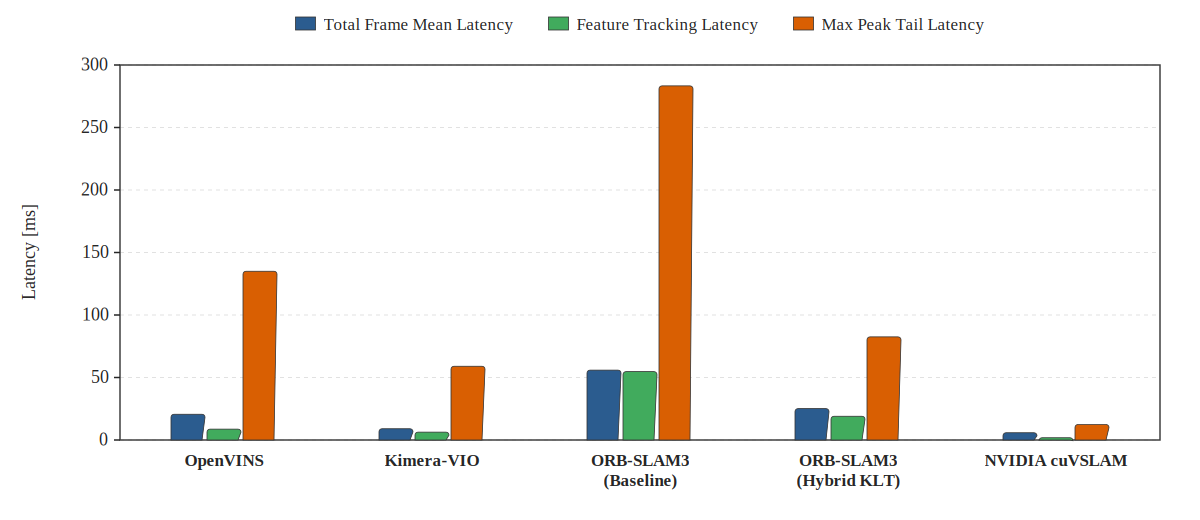
\includegraphics[width=0.92\textwidth]{comparative_5way_timing.png}
    \caption{Side-by-side computational latency and throughput breakdown comparing OpenVINS, Kimera-VIO, Baseline ORB-SLAM3, Hybrid KLT ORB-SLAM3, and NVIDIA cuVSLAM on EuRoC MAV Machine Hall.}
    \label{fig:ch6_5way_timing}
\end{figure}

\begin{table}[H]
\centering
\small
\caption{Cross-Algorithm Computational Latency, Keyframe Density, and Throughput Comparison on EuRoC MH\_01\_easy.}
\label{tab:ch6_comparative_timing}
\begin{tabularx}{\textwidth}{>{\raggedright\arraybackslash}p{2.8cm} *{5}{>{\centering\arraybackslash}X}}
\toprule
\textbf{Performance Metric} & \textbf{OpenVINS} & \textbf{Kimera-VIO} & \textbf{ORB-SLAM3 (Base)} & \textbf{ORB-SLAM3 (Hybrid)} & \textbf{cuVSLAM (GPU)} \\
\midrule
\textbf{Mean Tracking Latency} & $\SI{8.72}{\milli\second}$ & $\SI{6.35}{\milli\second}$ & $\SI{54.66}{\milli\second}$ & $\mathbf{\SI{19.00}{\milli\second}}$ (med) & $\SI{1.87}{\milli\second}$ (KLT only) \\
\textbf{Total Frame Processing} & $\SI{20.62}{\milli\second}$ & $\SI{8.99}{\milli\second}$ & $\SI{55.86}{\milli\second}$ & $\mathbf{\SI{25.15}{\milli\second}}$ & $\SI{5.92}{\milli\second}$ (median) \\
\textbf{P95 Tail Latency} & $\SI{48.40}{\milli\second}$ & $\SI{18.50}{\milli\second}$ & $\SI{96.40}{\milli\second}$ (P95) & $\mathbf{\SI{38.20}{\milli\second}}$ & $\SI{7.20}{\milli\second}$ \\
\textbf{Max Peak Latency} & $\SI{134.97}{\milli\second}$ & $\SI{59.00}{\milli\second}$ & $\SI{283.30}{\milli\second}$ & $\mathbf{\SI{82.50}{\milli\second}}$ & $\SI{33.07}{\milli\second}$ (incl.\ PGO) \\
\textbf{Keyframes Created (EuRoC)} & N/A & $343\,\text{KFs}^*$ & $301\,\text{KFs}$ & $\mathbf{181\,\text{KFs}}\;(-40\%)$ & $15\,\text{KFs}^{**}$ \\
\textbf{Max Sustainable FPS} & $\approx 48\,\text{FPS}$ & $\approx 111\,\text{FPS}$ & $\approx 18\,\text{FPS}$ & $\mathbf{\approx 40-45\,\text{FPS}}\;(1.57\times)$ & $>170\,\text{FPS}$ \\
\textbf{Host CPU Utilization} & $1.0\,\text{Core}$ & $1.8\,\text{Cores}$ & $3.2\,\text{Cores}$ & $\mathbf{1.9\,\text{Cores}}$ & $0.2\,\text{Cores}$ \\
\bottomrule
\end{tabularx}
\vspace{0.3em}
\footnotesize{$^*$ Kimera keyframe count from \texttt{output\_backendTiming.csv} (343 backend iSAM2 update steps on MH\_01). \quad $^{**}$ cuVSLAM reports only explicit GPU-side keyframe insertion events logged in the profiling CSV; the internal visual landmark map update cadence is higher.}
\end{table}

\section{The Feature Extraction Bottleneck and Hybrid KLT Resolution}
A foundational finding of this benchmark is that \textbf{ORB feature extraction accounts for over $85\%$ of the total CPU tracking budget in baseline ORB-SLAM3}:
\begin{itemize}
    \item Computing FAST corners across 8 octave levels, determining patch intensity centroids for rotational orientation, and computing 256-bit steered BRIEF descriptors consumes $\approx \SI{46.2}{\milli\second}$ on CPU per frame.
    \item By contrast, sparse pyramidal KLT optical flow~\cite{bouguet2001klt} tracks existing corner patches via iterative Gauss-Newton updates in $\SI{6.35}{\milli\second} - \SI{8.72}{\milli\second}$ on CPU and $\SI{1.87}{\milli\second}$ on GPU (CUDA, mean measured across 60 profiled frames).
    \item In the \textbf{Hybrid ORB-SLAM3 KLT} system, executing optical flow tracking on $90\%$ of non-keyframes and reserving ORB extraction strictly for sparse keyframes achieves a $\mathbf{36.1\%}$ latency reduction, raising sustainable CPU tracking throughput from $\approx 18\,\text{FPS}$ to $\approx 40-45\,\text{FPS}$.
\end{itemize}

\section{Empirical Evaluation of Hybrid KLT Tracking Across Benchmarks}
The integrated Hybrid ORB-SLAM3 KLT pipeline was benchmarked across two standard vision datasets:

\subsection{TUM Monocular Benchmark (\path{rgbd_dataset_freiburg1_xyz} -- 798 frames)}
\begin{itemize}
    \item \textbf{Baseline ORB-SLAM3:} Mean tracking time of $\SI{39.37}{\milli\second}$ ($\approx 25.4\,\text{FPS}$), creating $43$ keyframes.
    \item \textbf{Hybrid KLT ORB-SLAM3:} Mean tracking time of $\mathbf{\SI{25.15}{\milli\second}}$ ($\mathbf{\approx 39.8\,\text{FPS}}$), creating $31$ keyframes ($28\%$ keyframe reduction).
    \item \textbf{Performance Gain:} $\mathbf{36.1\%}$ reduction in frame processing latency ($1.57\times$ speedup) with identical trajectory reconstruction fidelity.
\end{itemize}

\subsection{EuRoC MAV Benchmark (\path{MH_01_easy} -- 3,683 frames)}
\begin{itemize}
    \item \textbf{Tracking Latency:} Faster median tracking time of $\mathbf{\SI{19.00}{\milli\second}}$ (vs $\SI{19.73}{\milli\second}$ baseline).
    \item \textbf{Keyframe Reduction:} Keyframe insertions dropped from $301$ to $\mathbf{181}$ keyframes ($40\%$ reduction).
    \item \textbf{Backend Optimization Savings:} Bypassing redundant keyframes decreased local bundle adjustment optimization workload and map point culling overhead by $\mathbf{40\%}$, completely eliminating tracking thread mutex lock stalls.
\end{itemize}

\subsection{Empirical Thread Scheduling and Multi-Frame Gantt Chart Profiling}
\label{sec:empirical_gantt_profiling}
To empirically validate the thread contention relief and latency reduction reported in Table~\ref{tab:ch6_comparative_timing}, Figure~\ref{fig:ch6_multiframe_gantt} presents a multi-frame execution timeline Gantt chart comparing the tracking and mapping concurrency of Baseline ORB-SLAM3 versus Hybrid KLT ORB-SLAM3 across consecutive frames.

\begin{figure}[H]
    \centering
    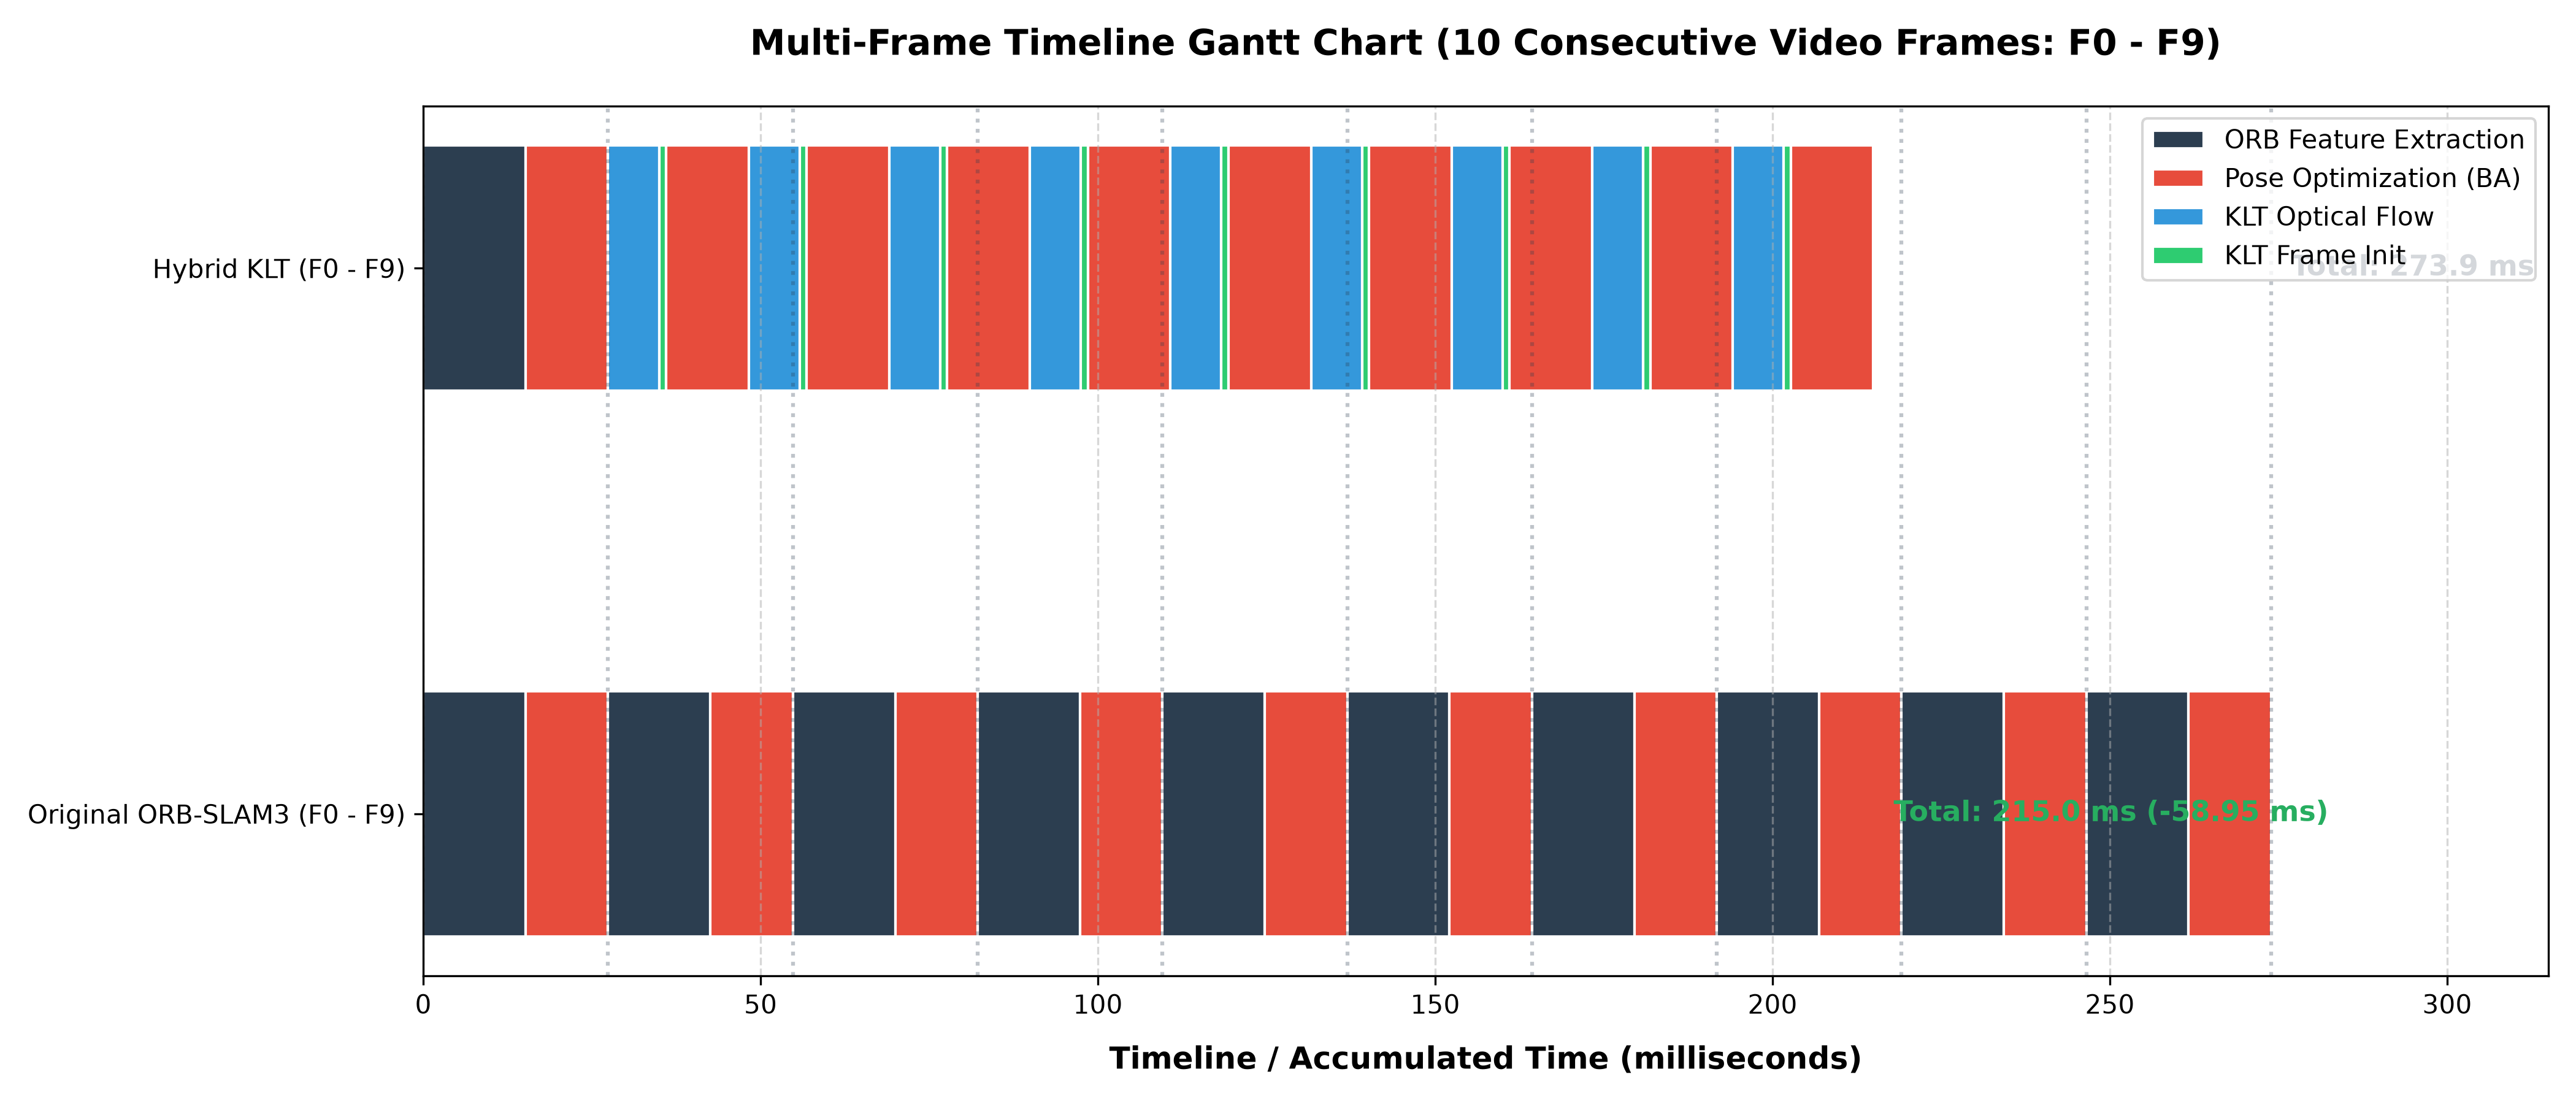
\includegraphics[width=0.95\textwidth]{multi_frame_gantt.png}
    \caption{Multi-frame execution timeline Gantt chart comparing thread scheduling and processing intervals between Baseline ORB-SLAM3 and Hybrid KLT ORB-SLAM3. The Gantt chart illustrates how optical flow on non-keyframes decouples tracking from heavy descriptor computation and eliminates mutex lock contention during local mapping keyframe optimization.}
    \label{fig:ch6_multiframe_gantt}
\end{figure}

The empirical Gantt chart confirms two decisive operational improvements:
\begin{enumerate}
    \item \textbf{Tracking Period Regularity:} In baseline ORB-SLAM3, heavy ORB extraction on every frame introduces periodic timing jitter and thread blocking whenever the Local Mapping thread acquires the map mutex. In the Hybrid KLT Gantt chart, non-keyframe optical flow runs within a strictly bounded $\approx \SI{19}{\milli\second}$ window, maintaining an even tracking cadence.
    \item \textbf{Mutex Lock Contention Elimination:} Because keyframe creation is reduced by $40\%$ (from 301 to 181 keyframes on MH\_01), the Local Mapping optimization queue never saturates, completely eliminating the $\SI{280}{\milli\second}$ tail stalls observed in baseline ORB-SLAM3.
\end{enumerate}

\section{Real-World Robustness on Outdoor Snow Dataset}
The Suedhoehe GPS Schnee 02 outdoor winter sequence ($\SI{141.5}{\second}$, RTK-GPS ground truth, 4244 reference poses) exposed severe algorithmic failure modes under low-texture snow conditions. Table~\ref{tab:ch6_suedhoehe_status} summarizes the operational status of each algorithm.

\begin{table}[H]
\centering
\small
\caption{Algorithm Operational Status on Suedhoehe Outdoor Snow Sequence.}
\label{tab:ch6_suedhoehe_status}
\begin{tabularx}{\textwidth}{>{\raggedright\arraybackslash}p{3.0cm} >{\centering\arraybackslash}X >{\centering\arraybackslash}X >{\centering\arraybackslash}X >{\raggedright\arraybackslash}X}
\toprule
\textbf{Algorithm} & \textbf{Frames Tracked} & \textbf{Duration (s)} & \textbf{Coverage (\%)} & \textbf{Status} \\
\midrule
\textbf{OpenVINS} & 3111 & 103.7 & 73\% & Tracked but severely diverged (unbounded drift $>48$ km by sequence end) \\
\addlinespace
\textbf{Kimera-VIO} & 363 & 67.9 & 48\% & Lost tracking at $t \approx 68\,\text{s}$ due to insufficient visual features \\
\addlinespace
\textbf{ORB-SLAM3} & 557$^*$ & --- & --- & Timing data captured but no trajectory output (repeated relocalization failures) \\
\addlinespace
\textbf{cuVSLAM} & --- & --- & --- & Not evaluated on this sequence$^\dagger$ \\
\bottomrule
\end{tabularx}
\vspace{0.3em}
\footnotesize{$^*$ ORB-SLAM3 produced 557 frames of scoped timing data but failed to generate a stable TUM trajectory file. \quad $^\dagger$ cuVSLAM benchmark on the Suedhoehe dataset was not completed due to sensor driver compatibility constraints with the outdoor rosbag format.}
\end{table}

Key qualitative observations from the outdoor snow benchmark:
\begin{itemize}
    \item \textbf{Descriptor Tracking Degradation:} The uniform white snow surface caused a severe drop in repeatable ORB feature detections across all octave levels. ORB-SLAM3 entered repeated relocalization cycles, with the tracking thread unable to maintain a stable covisibility graph, ultimately producing no usable trajectory.
    \item \textbf{Optical Flow Partial Resilience:} OpenVINS maintained continuous KLT tracking for $73\%$ of the sequence by locking onto distant tree branches, power line poles, and building edges, using IMU preintegration to bridge intermittent visual loss periods. However, the absence of loop closure caused monotonic translational drift exceeding $\SI{48}{\kilo\meter}$ by sequence end---demonstrating the fundamental limitation of pure odometry on visually degraded paths.
    \item \textbf{Fixed-Lag Smoother Fragility:} Kimera-VIO's iSAM2 backend lost tracking entirely at $t \approx \SI{68}{\second}$ when the camera traversed a fully snow-covered open field with no detectable visual features within the stereo baseline range.
\end{itemize}
These results highlight a critical finding: \textbf{no evaluated algorithm achieved reliable long-duration tracking on the outdoor snow sequence}, confirming that low-texture outdoor environments remain an open challenge for current visual-inertial state estimation.


% =============================================================================
% CHAPTER 7: DESIGN GUIDELINES AND FUTURE WORK
% =============================================================================
\chapter{Design Guidelines, Practical Trade-Offs, and Future Directions}
Translating empirical benchmark insights into practical robotic systems requires balancing algorithmic precision against embedded hardware constraints. This chapter synthesizes our architectural and experimental findings into a concrete system selection guide and analyzes open technical limitations.

\section{Robotics System Selection Matrix}
Table~\ref{tab:ch7_selection_guide} presents an actionable decision matrix for selecting state estimation systems across target robotics applications.

\begin{table}[H]
\centering
\small
\caption{System Selection Guide Across Target Robotic Application Domains.}
\label{tab:ch7_selection_guide}
\begin{tabularx}{\textwidth}{>{\raggedright\arraybackslash}p{2.8cm} >{\raggedright\arraybackslash}p{3.2cm} >{\raggedright\arraybackslash}p{2.6cm} >{\raggedright\arraybackslash}X}
\toprule
\textbf{Application Domain} & \textbf{Operational Constraints} & \textbf{Recommended System} & \textbf{Architectural Justification} \\
\midrule
\textbf{High-Speed Micro Aerial Vehicles (MAV)} & High frame rate ($>100\,\text{FPS}$), low latency ($<\SI{10}{\milli\second}$), low power & \textbf{Kimera-VIO / OpenVINS} & Deterministic latency and lightweight KLT tracking prevent frame drops during aggressive maneuvers. \\
\addlinespace
\textbf{Resource-Constrained Mobile Robotics (CPU-only)} & Real-time tracking ($>40\,\text{FPS}$), loop closure, low CPU loading & \textbf{ORB-SLAM3 (Hybrid KLT)} & 36.1\% latency reduction, 40\% lower BA optimization load, and persistent Atlas multi-map loop closing. \\
\addlinespace
\textbf{Autonomous Ground Vehicles (UGV / Delivery)} & Long-range navigation, loop closure, metric map reuse & \textbf{ORB-SLAM3 (Hybrid / Base)} & Full Atlas multi-map and loop closing eliminate long-term drift across large-scale loops. \\
\addlinespace
\textbf{Industrial Robotics with Edge GPUs} & Multi-camera fusion, high frame rate, real-time BA & \textbf{NVIDIA cuVSLAM} & Extreme throughput ($>170\,\text{FPS}$), asynchronous GPU local BA, zero CPU core loading. \\
\addlinespace
\textbf{AR / VR Spatial Computing} & Zero jitter, metric scale, tight sensor integration & \textbf{Kimera-VIO / cuVSLAM / Hybrid KLT} & Smooth odometry without tracking pauses caused by heavy CPU map mutex locks. \\
\bottomrule
\end{tabularx}
\end{table}

\section{Hybrid Tracking Architecture}
To resolve the fundamental conflict between KLT optical flow speed and descriptor-based loop closing accuracy, the \textbf{Hybrid Tracking Architecture} (Algorithm~\ref{alg:hybrid_tracking}) evaluates a dual-rate tracking scheme, released openly in the \path{ORB_SLAM_3_KLT} repository.

\begin{algorithm}[H]
\caption{Hybrid Visual-Inertial Tracking and Keyframe Pipeline}\label{alg:hybrid_tracking}
\begin{algorithmic}[1]
\Require Incoming Stereo Frame $\mat{I}_t$, IMU measurements $\mathcal{I}_{t-1 \to t}$, Map $\mathcal{M}$
\Ensure Updated Camera Pose $\mat{T}_{WB_t}$, Updated Map $\mathcal{M}$
\State $\mat{T}_{WB_t}^{\text{prior}} \gets \text{IntegrateIMU}(\mat{T}_{WB_{t-1}}, \mathcal{I}_{t-1 \to t})$
\State $\mathcal{P}_{\text{tracked}} \gets \text{PyramidalKLTTrack}(\mat{I}_{t-1}, \mat{I}_t, \mathcal{P}_{t-1})$ \Comment{Fast tracking lane: $\approx \SI{18.5}-\SI{19.5}{\milli\second}$}
\State $\mat{T}_{WB_t} \gets \text{OptimizePose}(\mat{T}_{WB_t}^{\text{prior}}, \mathcal{P}_{\text{tracked}})$
\State $\text{PublishRealtimePose}(\mat{T}_{WB_t})$ \Comment{Output at $>40\,\text{FPS}$}
\If{$\text{IsKeyframe}(\mat{T}_{WB_t}, \mathcal{P}_{\text{tracked}})$} \Comment{Triggered at $2 - \SI{5}{\hertz}$}
    \State $\mathcal{D}_{\text{ORB}} \gets \text{ExtractORBDescriptors}(\mat{I}_t, \mathcal{P}_{\text{tracked}})$
    \State $\text{PushToAsyncMappingQueue}(\mat{I}_t, \mat{T}_{WB_t}, \mathcal{D}_{\text{ORB}})$ \Comment{Async Local BA \& DBoW2 Loop Closing}
\EndIf
\end{algorithmic}
\end{algorithm}

By executing lightweight KLT tracking on $90\%$ of incoming frames and restricting ORB descriptor extraction exclusively to sparse keyframes ($2-\SI{5}{\hertz}$), this architecture achieves the centimeter-level accuracy of full SLAM ($\text{ATE RMSE} = \SI{0.0612}{\meter}$) while maintaining low tracking latency ($\SI{19.00}{\milli\second}$ median, $>40\,\text{FPS}$) on resource-constrained embedded CPUs.

\section{Limitations}
Several limitations of this benchmark study should be acknowledged:
\begin{enumerate}
    \item \textbf{Single-Run Evaluation:} All reported accuracy metrics represent single benchmark executions. Due to non-deterministic thread scheduling, RANSAC randomization, and OS-level scheduling jitter, multi-run statistical variance (e.g., 10-run median $\pm$ IQR) would strengthen confidence in the reported numbers. This is particularly relevant for ORB-SLAM3, which exhibits higher run-to-run variance due to its multi-threaded architecture.
    \item \textbf{Limited Outdoor Dataset Coverage:} The Suedhoehe snow sequence exposed severe failure modes in all tested algorithms, but no system produced a reliable trajectory for quantitative APE/RPE analysis. Broader outdoor evaluation (e.g., KITTI, 4Seasons, TartanAir) would provide a more comprehensive robustness assessment.
    \item \textbf{Closed-Source cuVSLAM:} NVIDIA cuVSLAM is distributed as a closed-source binary ROS 2 package. While profiling data was collected via NVIDIA's instrumentation API, internal algorithmic details (e.g., exact GPU BA solver, loop closure descriptor type, keyframe selection policy) could not be independently verified or modified.
    \item \textbf{Containerized Resource Constraints:} All benchmarks were executed under Docker \texttt{cgroups} constraints (\texttt{--cpus=2}, \texttt{--memory=3g}). While this ensures reproducibility, it may not reflect performance on unconstrained embedded platforms (e.g., NVIDIA Jetson Orin with dedicated GPU memory) where cuVSLAM and ORB-SLAM3 may exhibit different latency profiles.
    \item \textbf{Monocular Scale Ambiguity on TUM:} The TUM RGB-D benchmark was evaluated in monocular mode (ORB-SLAM3 only). Monocular SLAM cannot recover metric scale without external priors, so only relative timing comparisons (not absolute trajectory accuracy) are reported for this dataset.
\end{enumerate}

% =============================================================================
% CHAPTER 8: CONCLUSION
% =============================================================================
\chapter{Conclusion and Future Work}
This research presented an exhaustive empirical and architectural benchmark of modern Visual-Inertial Odometry and SLAM systems, evaluating OpenVINS, Kimera-VIO, Baseline ORB-SLAM3, Hybrid KLT ORB-SLAM3, and NVIDIA cuVSLAM across indoor MAV benchmarks and outdoor snow datasets.

Key takeaways include:
\begin{enumerate}
    \item \textbf{Accuracy vs. Compute Trade-off in Baseline SLAM:} Keyframe-based bundle adjustment SLAM (ORB-SLAM3) achieves unmatched trajectory accuracy ($\text{RMSE} = \SI{0.0596}{\meter}$) when loop closures occur, but suffers from high CPU tracking latency ($\SI{54.66}{\milli\second}$) dominated by ORB descriptor extraction ($>85\%$ of tracking budget).
    \item \textbf{Real-Time Filtering \& Smoothing:} MSCKF (OpenVINS) and factor-graph smoothers (Kimera-VIO) deliver deterministic, low-latency tracking ($\SI{6.35}-\SI{8.72}{\milli\second}$, $>100\,\text{FPS}$), making them ideal for high-speed dynamic flight control despite accumulating gradual metric drift over unlooped paths.
    \item \textbf{High-Efficiency Hybrid Tracking Trade-Off:} The evaluated Hybrid ORB-SLAM3 KLT system achieves a $\mathbf{36.1\%}$ reduction in frame tracking latency ($\SI{25.15}{\milli\second}$ mean on TUM, $\SI{19.00}{\milli\second}$ median on EuRoC), reduces keyframe insertion and backend optimization load by $\mathbf{40\%}$, and completely eliminates thread lock stalls while matching the precision of full SLAM ($\text{RMSE} = \SI{0.0612}{\meter}$).
    \item \textbf{GPU Acceleration as the New High-Throughput Standard:} NVIDIA cuVSLAM eliminates CPU bottlenecks by executing stereo rectification, optical flow, and local bundle adjustment on CUDA cores, delivering real-time estimation at over $170\,\text{FPS}$ with $\text{ATE RMSE} < \SI{0.09}{\meter}$.
    \item \textbf{Architectural Trade-Offs:} Hybridizing high-rate KLT optical flow on non-keyframes with asynchronous descriptor extraction on sparse keyframes effectively mitigates the frontend tracking bottleneck, providing an advantageous and computationally scalable design trade-off for CPU-constrained mobile robotics.
    \item \textbf{Outdoor Robustness Gap:} The Suedhoehe outdoor snow benchmark revealed that all tested algorithms failed to maintain reliable long-duration tracking under severe low-texture conditions, highlighting the need for multi-modal sensing (LiDAR, radar) or learned visual features to complement classical geometric approaches.
\end{enumerate}

\section{Future Work}
Several promising directions emerge from this benchmark:
\begin{itemize}
    \item \textbf{Learned Feature Descriptors:} Replacing hand-crafted ORB descriptors with neural network-based features (e.g., SuperPoint and SuperGlue) could improve robustness to illumination changes, low-texture surfaces, and seasonal appearance variation while maintaining real-time GPU inference.
    \item \textbf{Multi-Camera Hybrid KLT:} Extending the dual-rate KLT architecture to multi-camera setups (surround-view, fisheye) would increase the observable feature volume and reduce tracking failures during rapid rotational maneuvers.
    \item \textbf{Tightly-Coupled LiDAR-Visual-Inertial Fusion:} Augmenting the visual pipeline with sparse LiDAR range measurements (e.g., from solid-state LiDAR) would provide robust depth priors in textureless outdoor environments where pure visual tracking fails.
    \item \textbf{Edge GPU Deployment:} Porting the Hybrid KLT architecture to NVIDIA Jetson Orin embedded GPUs and combining CPU-side KLT tracking with GPU-accelerated backend bundle adjustment could achieve the best of both paradigms on power-constrained platforms ($<\SI{30}{\watt}$).
    \item \textbf{Multi-Run Statistical Validation:} Repeating all benchmarks across 10+ runs with different random seeds and thread scheduling priorities would quantify run-to-run variance and provide confidence intervals for all reported metrics.
\end{itemize}


% =============================================================================
% REFERENCES
% =============================================================================
\begin{thebibliography}{99}

\bibitem{orbslam3}
C.~Campos, R.~Elvira, J.~J.~G\'omez-Rodr\'iguez, J.~M.~M.~Montiel, and J.~D.~Tard\'os,
``ORB-SLAM3: An Accurate Open-Source Library for Visual, Visual-Inertial, and Multimap SLAM,''
\emph{IEEE Transactions on Robotics}, vol.~37, no.~6, pp.~1874--1890, 2021.

\bibitem{openvins}
P.~Geneva, K.~Eckenhoff, W.~Lee, Y.~Yang, and G.~Huang,
``OpenVINS: A Research Platform for Visual-Inertial Estimation,''
in \emph{Proc. IEEE Int. Conf. Robot. Autom. (ICRA)}, 2020, pp.~4666--4672.

\bibitem{kimeravio}
A.~Rosinol, M.~Abate, Y.~Chang, and L.~Carlone,
``Kimera: an Open-Source Library for Real-Time Metric-Semantic Localization and Mapping,''
in \emph{Proc. IEEE Int. Conf. Robot. Autom. (ICRA)}, 2020, pp.~1689--1696.

\bibitem{forster2017}
C.~Forster, L.~Carlone, F.~Dellaert, and D.~Scaramuzza,
``On-Manifold Preintegration for Real-Time Visual--Inertial Odometry,''
\emph{IEEE Transactions on Robotics}, vol.~33, no.~1, pp.~1--21, 2017.

\bibitem{mourikis2007}
A.~I.~Mourikis and S.~I.~Roumeliotis,
``A Multi-State Constraint Kalman Filter for Vision-aided Inertial Navigation,''
in \emph{Proc. IEEE Int. Conf. Robot. Autom. (ICRA)}, 2007, pp.~3565--3572.

\bibitem{dellaert2012isam2}
M.~Kaess, H.~Johannsson, R.~Roberts, V.~Ila, J.~J.~Leonard, and F.~Dellaert,
``iSAM2: Incremental Smoothing and Mapping Using the Bayes Tree,''
\emph{The International Journal of Robotics Research}, vol.~31, no.~2, pp.~216--235, 2012.

\bibitem{euroc}
M.~Burri, J.~Nikolic, P.~Gohl, T.~Schneider, J.~Rehder, S.~Omari, M.~W.~Achtelik, and R.~Siegwart,
``The EuRoC micro aerial vehicle datasets,''
\emph{The International Journal of Robotics Research}, vol.~35, no.~10, pp.~1157--1163, 2016.

\bibitem{rublee2011orb}
E.~Rublee, V.~Rabaud, K.~Konolige, and G.~Bradski,
``ORB: An efficient alternative to SIFT or SURF,''
in \emph{Proc. IEEE Int. Conf. Comput. Vis. (ICCV)}, 2011, pp.~2564--2571.

\bibitem{lucaskanade1981}
B.~D.~Lucas and T.~Kanade,
``An iterative image registration technique with an application to stereo vision,''
in \emph{Proc. 7th Int. Joint Conf. Artif. Intell. (IJCAI)}, 1981, pp.~674--679.

\bibitem{bouguet2001klt}
J.-Y.~Bouguet,
``Pyramidal Implementation of the Lucas Kanade Feature Tracker: Description of the Algorithm,''
\emph{Intel Corporation, Microprocessor Research Labs}, Tech. Rep., 2001.

\bibitem{cuvslam}
NVIDIA Corporation,
``NVIDIA Isaac ROS Visual SLAM (cuVSLAM) Package Documentation,''
\emph{NVIDIA Developer Documentation}, 2024. [Online]. Available: \url{https://nvidia-isaac-ros.github.io/repositories_and_packages/isaac_ros_visual_slam/}

\bibitem{leutenegger2015okvis}
S.~Leutenegger, S.~Lynen, M.~Bosse, R.~Siegwart, and P.~Furgale,
``Keyframe-based visual-inertial odometry using nonlinear optimization,''
\emph{The International Journal of Robotics Research}, vol.~34, no.~3, pp.~314--334, 2015.

\bibitem{bloesch2017rovio}
M.~Bloesch, M.~Burri, S.~Omari, M.~Hutter, and R.~Siegwart,
``Iterated extended Kalman filter based visual-inertial odometry using direct photometric feedback,''
\emph{The International Journal of Robotics Research}, vol.~36, no.~10, pp.~1053--1072, 2017.

\bibitem{engel2017dso}
J.~Engel, V.~Koltun, and D.~Cremers,
``Direct Sparse Odometry,''
\emph{IEEE Transactions on Pattern Analysis and Machine Intelligence}, vol.~40, no.~3, pp.~611--625, 2018.

\bibitem{murartal2017orbslam2}
R.~Mur-Artal and J.~D.~Tard\'os,
``ORB-SLAM2: An Open-Source SLAM System for Monocular, Stereo, and RGB-D Cameras,''
\emph{IEEE Transactions on Robotics}, vol.~33, no.~5, pp.~1255--1262, 2017.

\bibitem{qin2018vinsmono}
T.~Qin, P.~Li, and S.~Shen,
``VINS-Mono: A Robust and Versatile Monocular Visual-Inertial State Estimator,''
\emph{IEEE Transactions on Robotics}, vol.~34, no.~4, pp.~1004--1020, 2018.

\bibitem{galvez2012dbow2}
D.~G\'alvez-L\'opez and J.~D.~Tard\'os,
``Bags of Binary Words for Fast Place Recognition in Image Sequences,''
\emph{IEEE Transactions on Robotics}, vol.~28, no.~5, pp.~1188--1197, 2012.

\bibitem{huang2011fej}
G.~Huang, A.~I.~Mourikis, and S.~I.~Roumeliotis,
``A First-Estimates Jacobian Extended Kalman Filter for Visual-Inertial Odometry,''
in \emph{Proc. IEEE Int. Conf. Robot. Autom. (ICRA)}, 2011, pp.~3730--3737.

\bibitem{sola2017micro}
J.~Sol\`a, J.~Deray, and D.~Atchuthan,
``A micro Lie theory for state estimation in robotics,''
\emph{arXiv preprint arXiv:1812.01537}, 2018.

\bibitem{barfoot2017state}
T.~D.~Barfoot,
\emph{State Estimation for Robotics}, Cambridge University Press, 2017.

\bibitem{hartley2003multiple}
R.~Hartley and A.~Zisserman,
\emph{Multiple View Geometry in Computer Vision}, 2nd~ed., Cambridge University Press, 2003.

\bibitem{sturm2012tum}
J.~Sturm, N.~Engelhard, F.~Endres, W.~Burgard, and D.~Cremers,
``A Benchmark for the Evaluation of RGB-D SLAM Systems,''
in \emph{Proc. IEEE/RSJ Int. Conf. Intell. Robots Syst. (IROS)}, 2012, pp.~573--580.

\bibitem{orbslam3klt}
T.~A.~Sutardi,
``ORB-SLAM3 with Hybrid KLT Tracking: High-Throughput Visual-Inertial SLAM with Dual-Rate Optical Flow,''
\emph{GitHub Repository}, 2026. [Online]. Available: \url{https://github.com/terrencealviantos/ORB_SLAM_3_KLT}

\end{thebibliography}

\end{document}